% Please don't change anything in the documentclass below:
\documentclass[compsoc, conference, 10pt, times]{IEEEtran}

% We recommend using these packages as below, but if you have a good reason and want to change these, you can.
\usepackage{cite}
\usepackage{amsmath,amssymb,amsfonts}
% \usepackage{algorithmic}
\usepackage{graphicx}
\usepackage{tcolorbox}
\usepackage{threeparttable}
\usepackage{booktabs}
\usepackage{adjustbox}
\usepackage{enumitem}
% \usepackage[dvipsnames]{xcolor}
\usepackage{textcomp,amssymb}
\usepackage{diagbox}
\usepackage{textcomp}
% \usepackage[svgnames]{xcolor}
% \def\BibTeX{{\rm B\kern-.05em{\sc i\kern-.025em b}\kern-.08em
%     T\kern-.1667em\lower.7ex\hbox{E}\kern-.125emX}}
\usepackage{textcomp}
\usepackage[linesnumbered,ruled,vlined]{algorithm2e}
\usepackage{algpseudocode}
\usepackage{multirow}
\usepackage{makecell}
\usepackage{array}
\usepackage{wrapfig}
\usepackage{tikz}
\newcommand*\circled[1]{\tikz[baseline=(char.base)]{
            \node[shape=circle,draw,inner sep=0.1pt] (char) {#1};}}
\renewcommand{\algorithmicrequire}{\textbf{INPUT:}}
\renewcommand{\algorithmicensure}{\textbf{OUTPUT:}}
\newcommand{\bheading}[1]{{\vspace{2pt}\noindent{\textbf{#1}}\hspace{2pt}}}
\newcommand{\fixme}[1]{\textbf{\textcolor{red}{[FIXME: #1]}}}

\newcommand{\halfcirc}{\raisebox{-0.5mm}{\includegraphics[scale=0.025]{materials/halfcircle.png}}}
\newcommand{\emptycirc}{\raisebox{-0.5mm}{\includegraphics[scale=0.025]{materials/emptycircle.png}}}
\newcommand{\fullcirc}{\raisebox{-0.5mm}{\includegraphics[scale=0.025]{materials/fullcircle.png}}}
\newcommand{\voice}{\raisebox{-0.3mm}{\includegraphics[scale=0.03]{materials/voice.png}}}
\newcommand{\wave}{\raisebox{-0.3mm}{\includegraphics[scale=0.03]{materials/wave.png}}}
\newcommand{\laser}{\raisebox{-0.8mm}{\includegraphics[scale=0.03]{materials/laser.png}}}
\newcommand{\gps}{\raisebox{-0.6mm}{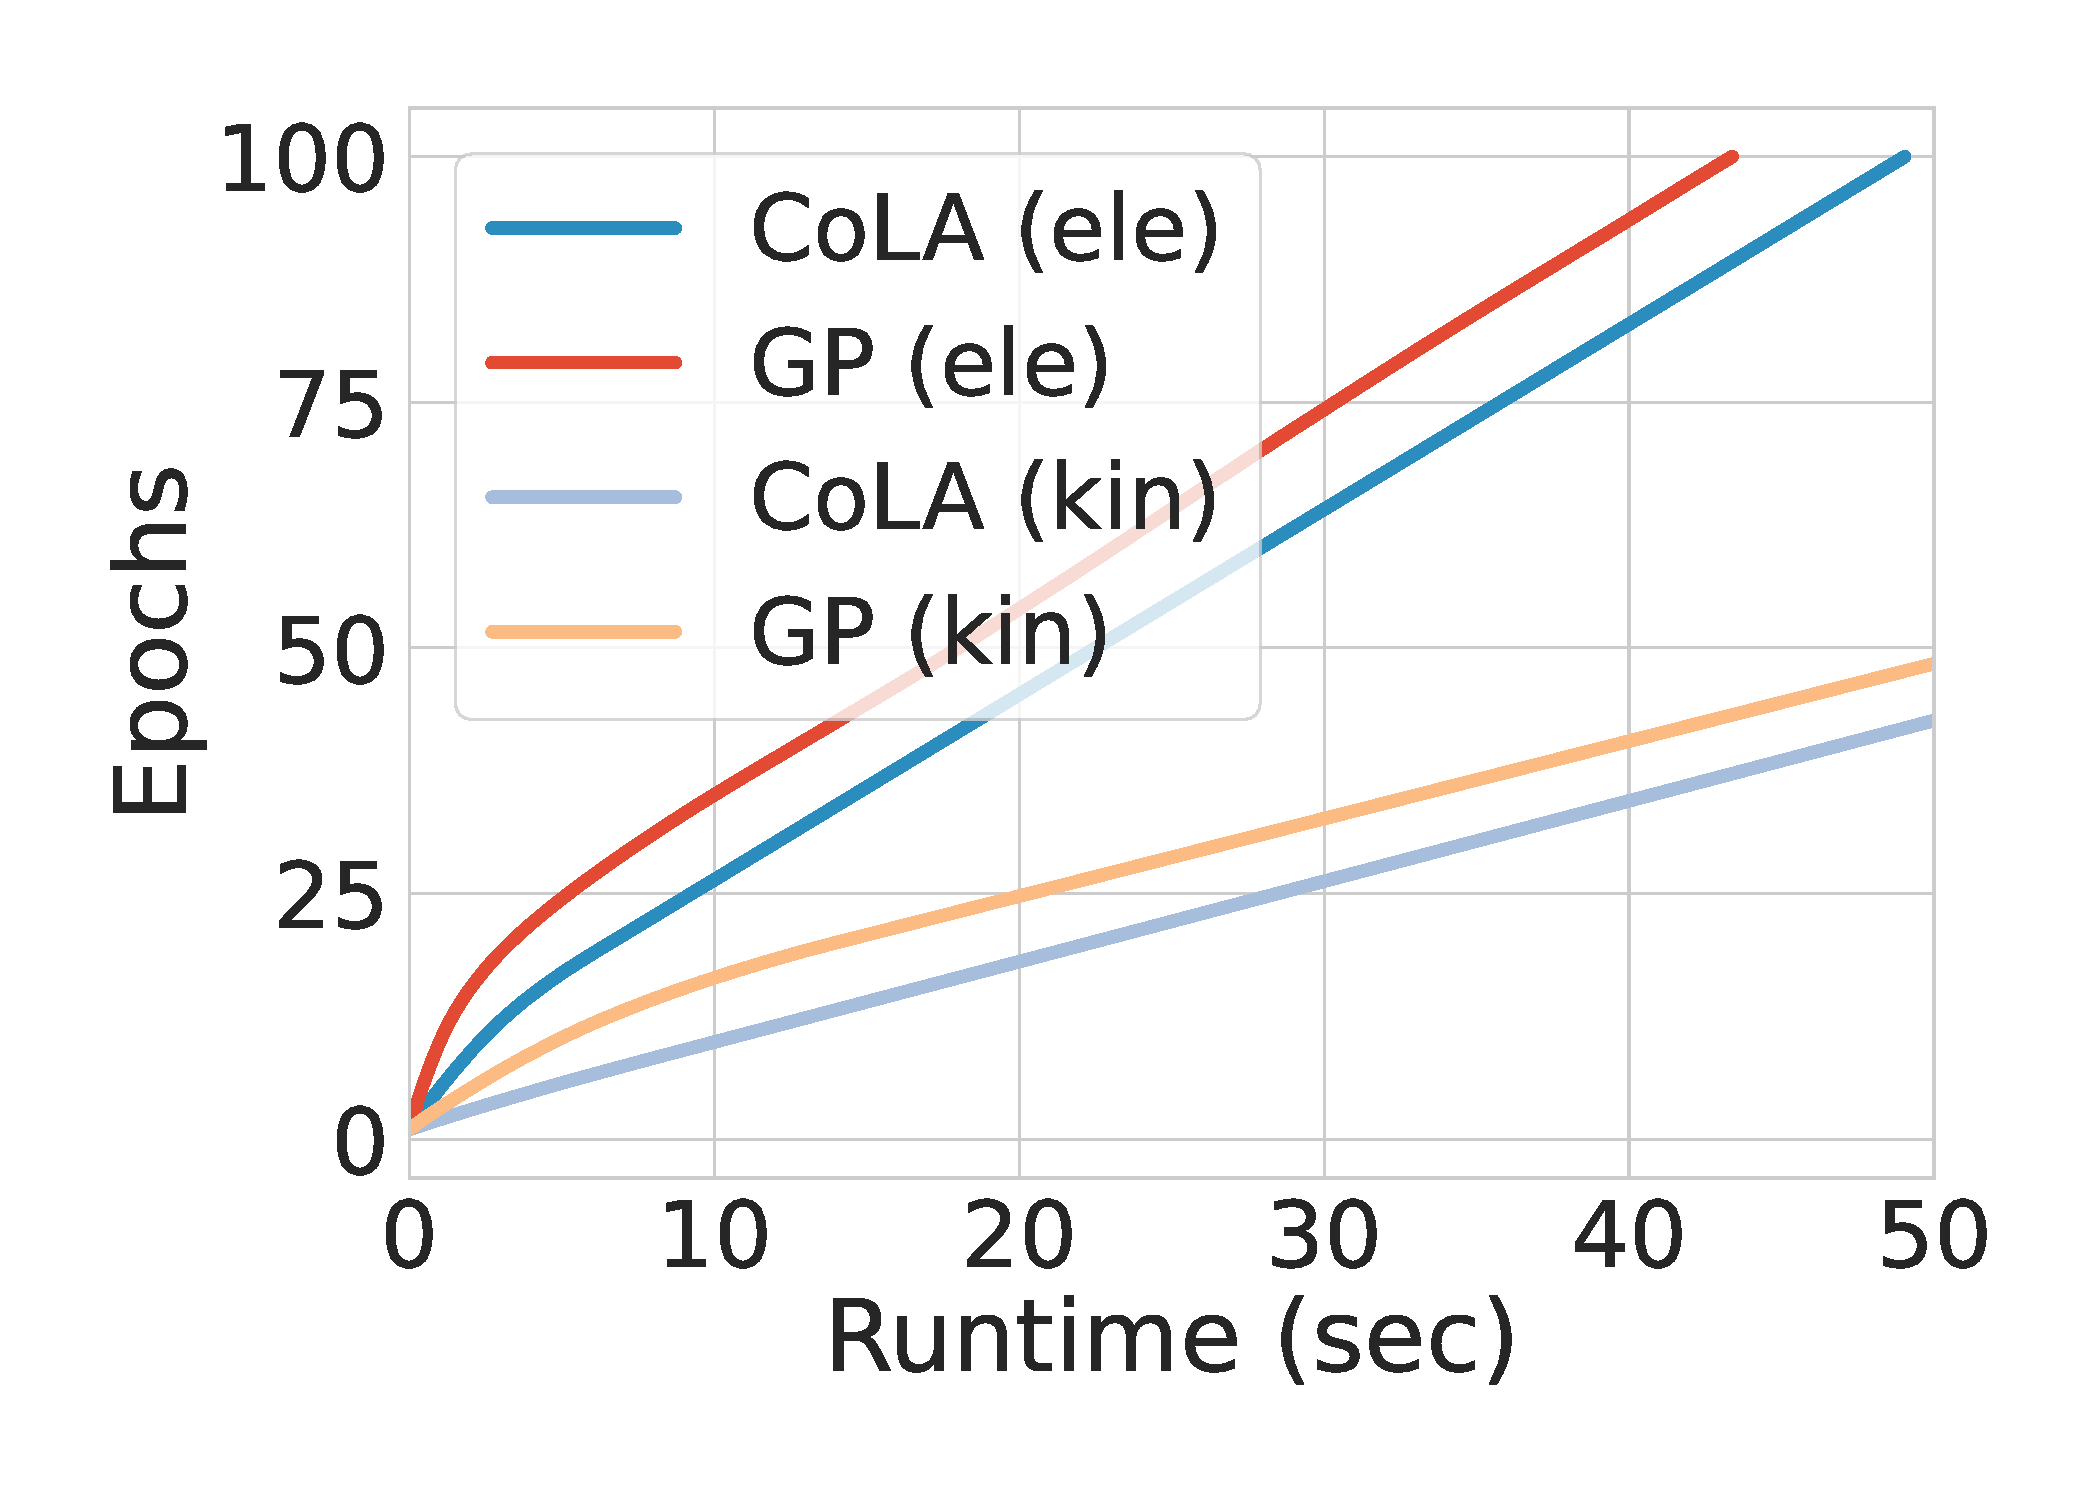
\includegraphics[scale=0.04]{materials/gps.png}}}
\newcommand{\shape}{\raisebox{-0.6mm}{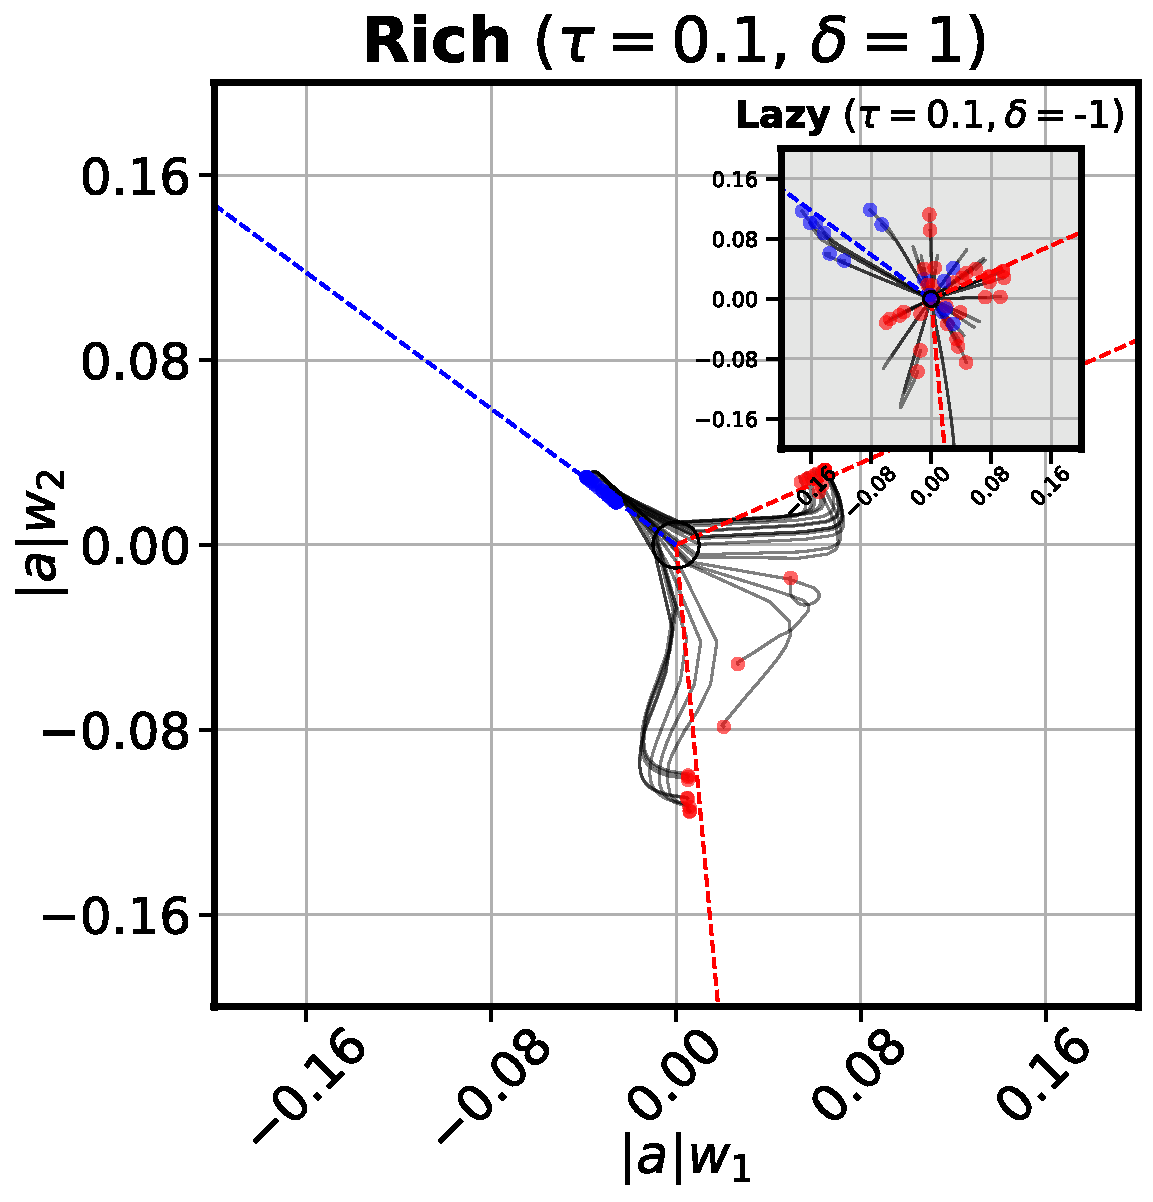
\includegraphics[scale=0.04]{materials/shape.png}}}
\newcommand{\sticker}{\raisebox{-0.6mm}{\includegraphics[scale=0.04]{materials/sticker.png}}}
\newcommand{\car}{\raisebox{-0.4mm}{\includegraphics[scale=0.06]{materials/car.png}}}
\newcommand{\drone}{\raisebox{-0.2mm}{\includegraphics[scale=0.035]{materials/drone.png}}}
\newcommand{\mb}{\raisebox{-0.4mm}{\includegraphics[scale=0.06]{materials/vacuum.png}}}
\newcommand{\indoor}{\raisebox{-1.0mm}{\includegraphics[scale=0.05]{materials/indoor.png}}}
\newcommand{\outdoor}{\raisebox{-0.7mm}{\includegraphics[scale=0.045]{materials/outdoor.png}}}
\newcommand{\atk}{\raisebox{-0.7mm}{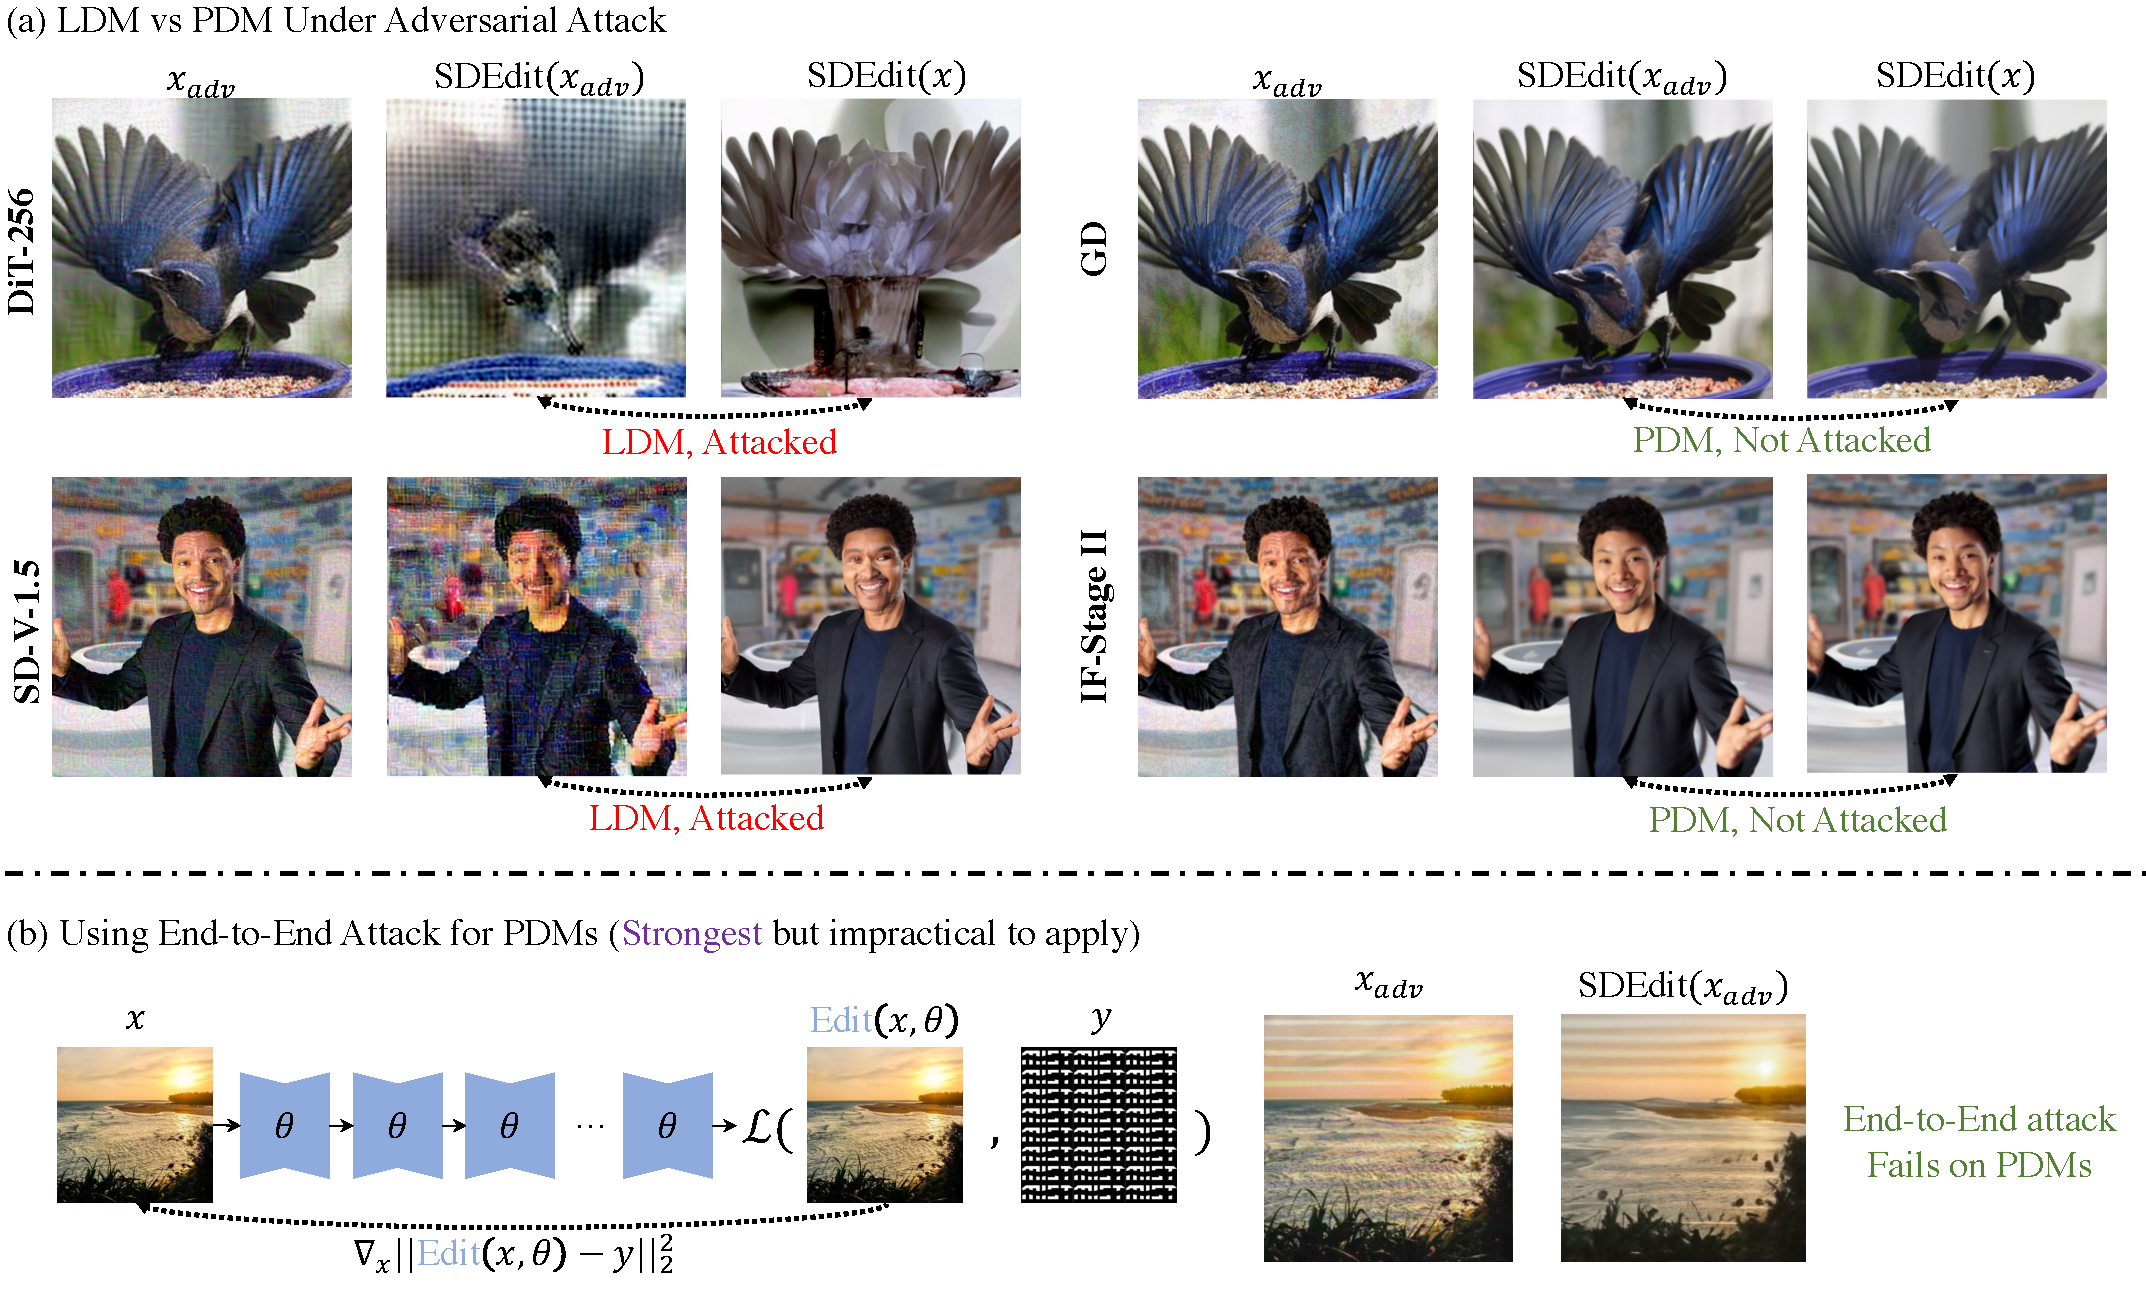
\includegraphics[scale=0.055]{materials/attack.png}}}
\newcommand{\ratk}{\raisebox{-0.7mm}{\includegraphics[scale=0.050]{materials/attack-red.png}}}
\newcommand{\batk}{\raisebox{-0.7mm}{\includegraphics[scale=0.050]{materials/attack-blue.png}}}
\newcommand{\gatk}{\raisebox{-0.7mm}{\includegraphics[scale=0.050]{materials/attack-green.png}}}
\newcommand{\mechanism}{\raisebox{-0.7mm}{\includegraphics[scale=0.045]{materials/tool-blue2.png}}}
\newcommand{\scenario}{\raisebox{-1.2mm}{\includegraphics[scale=0.065]{materials/scene-blue.png}}}

\usepackage{etoolbox}
\makeatletter
\patchcmd{\@makecaption}
  {\scshape}
  {}
  {}
  {}
\makeatother

\usepackage[font=normalsize]{caption}


\newcommand{\one}{\raisebox{-0.6mm}{\large{\ding{182}}}}
\newcommand{\two}{\raisebox{-0.6mm}{\large{\ding{183}}}}
\newcommand{\three}{\raisebox{-0.6mm}{\large{\ding{184}}}}
\newcommand{\four}{\raisebox{-0.6mm}{\large{\ding{185}}}}
\newcommand{\five}{\raisebox{-0.6mm}{\large{\ding{186}}}}
\newcommand{\six}{\raisebox{-0.6mm}{\large{\ding{187}}}}
\newcommand{\seven}{\raisebox{-0.6mm}{\large{\ding{188}}}}
\newcommand{\eight}{\raisebox{-0.6mm}{\large{\ding{189}}}}
\newcommand{\nine}{\raisebox{-0.6mm}{\large{\ding{190}}}}
\newcommand{\ten}{\raisebox{-0.6mm}{\large{\ding{191}}}}
\newcommand{\eleven}{\raisebox{-0.9mm}{
\includegraphics[scale=0.40]{materials/num/11.eps}}}

\newcommand{\arone}{\raisebox{-0.7mm}{\includegraphics[scale=0.50]{materials/ar/ar1.eps}}}
\newcommand{\artwo}{\raisebox{-0.7mm}{\includegraphics[scale=0.50]{materials/ar/ar2.eps}}}
\newcommand{\arthree}{\raisebox{-0.7mm}{\includegraphics[scale=0.50]{materials/ar/ar3.eps}}}
\newcommand{\arfour}{\raisebox{-0.7mm}{\includegraphics[scale=0.50]{materials/ar/ar4.eps}}}
\newcommand{\arfive}{\raisebox{-0.7mm}{\includegraphics[scale=0.50]{materials/ar/ar5.eps}}}
\newcommand{\arsix}{\raisebox{-0.7mm}{\includegraphics[scale=0.50]{materials/ar/ar6.eps}}}
\newcommand{\arseven}{\raisebox{-0.7mm}{\includegraphics[scale=0.50]{materials/ar/ar7.eps}}}
\newcommand{\areight}{\raisebox{-0.7mm}{\includegraphics[scale=0.50]{materials/ar/ar8.eps}}}
\newcommand{\arnine}{\raisebox{-0.7mm}{\includegraphics[scale=0.50]{materials/ar/ar9.eps}}}

% \usepackage{hyperref}
\usepackage[hidelinks]{hyperref}
\def\UrlBreaks{\do\A\do\B\do\C\do\D\do\E\do\F\do\G\do\H\do\I\do\J
\do\K\do\L\do\M\do\N\do\O\do\P\do\Q\do\R\do\S\do\T\do\U\do\V
\do\W\do\X\do\Y\do\Z\do\[\do\\\do\]\do\^\do\_\do\`\do\a\do\b
\do\c\do\d\do\e\do\f\do\g\do\h\do\i\do\j\do\k\do\l\do\m\do\n
\do\o\do\p\do\q\do\r\do\s\do\t\do\u\do\v\do\w\do\x\do\y\do\z
\do\.\do\@\do\\\do\/\do\!\do\_\do\|\do\;\do\>\do\]\do\)\do\,
\do\?\do\'\do+\do\=\do\#}

\usepackage{multirow}
\usepackage{pifont}
\usepackage{booktabs}
\usepackage{cleveref}
\usepackage{bbding}
\crefname{section}{§}{§§}
\usepackage{soul}
\usepackage{color}
\usepackage{xcolor}
\usepackage{colortbl}
\usepackage{setspace}
\usepackage{enumitem}
\usepackage{tcolorbox}
\usepackage{hhline}
\usepackage{changepage}
% \usepackage[flushleft]{threeparttable}
\usepackage{tabu}
\usepackage{subfigure}
% \usepackage{subfigure}
\usepackage{blindtext}
\usepackage{tcolorbox}
\usepackage{graphicx}
\usepackage{fontawesome}
\usepackage{cleveref}
\crefname{section}{§}{§§}
\Crefname{section}{§}{§§}
\newcommand{\yutong}[1]{\textcolor{red}{#1}}
% \newcommand{\xingshuo}[1]{{#1}}
% \renewcommand{\algorithmicrequire}{\textbf{Input:}}  % Use Input in the format of Algorithm  
% \renewcommand{\algorithmicensure}{\textbf{Output:}} % Use Output in the format of Algorithm
\newcommand{\zj}[1]{\textcolor{blue}{#1}}
\newcommand{\etal}{\textit{et al}.}
\newcommand{\el}{\textit{et al}.}
\newcommand{\ie}{\textit{i}.\textit{e}.}
\newcommand{\eg}{\textit{e}.\textit{g}.} 
\newcommand{\Tref}[1]{Table~\ref{#1}}
\newcommand{\Eref}[1]{Eq.~(\ref{#1})}
\newcommand{\Fref}[1]{Fig.~\ref{#1}}
\newcommand{\Sref}[1]{Sec.~\ref{#1}}
\newcommand{\Aref}[1]{Alg.~\ref{#1}}

\newenvironment{packeditemize}{
\begin{list}{$\bullet$}{
\setlength{\labelwidth}{8pt}
\setlength{\itemsep}{0pt}
\setlength{\leftmargin}{\labelwidth}
\addtolength{\leftmargin}{\labelsep}
\setlength{\parindent}{0pt}
\setlength{\listparindent}{\parindent}
\setlength{\parsep}{0pt}
\setlength{\topsep}{3pt}}}{\end{list}}
% \setlength{\tabcolsep}{1mm}
\hypersetup{
  colorlinks   = true,    % Colours links instead of ugly boxes
  urlcolor     = black,    % Colour for external hyperlinks
  linkcolor    = black,    % Colour of internal links
  citecolor    = red      % Colour of citations
}



\begin{document}


\title{Backdooring Textual Inversion for Concept Censorship}

% Submissions should be anonymized. See the CFP for details on how to anonymize your paper, including any references to your own work.
%\author{\em Anonymous Authors}

% The author information is skipped here, but can be used to include author information in the publication.
% \iffalse


\author{\IEEEauthorblockN{Yutong Wu$^{1}$, Jie Zhang$^{1*}$, Florian Kerschbaum$^{2}$, and Tianwei Zhang$^{1}$}
\IEEEauthorblockA{ $^{1}$Nanyang Technological University \\
$^{2}$University of Waterloo} \\}
% YUTONG002@e.ntu.edu.sg


% \author{\IEEEauthorblockN{Yutong Wu,}\textsuperscript{\rm 1}
% \IEEEauthorblockA{\textit{Nanyang Technological University} \\
% YUTONG002@e.ntu.edu.sg}
% \and
% \IEEEauthorblockN{Jie Zhang}
% \IEEEauthorblockA{\textit{Nanyang Technological University} \\
% jie\_zhang@ntu.edu.sg}
% \and
% \IEEEauthorblockN{Florian Kerschbaum}
% \IEEEauthorblockA{\textit{University of Waterloo} \\
% florian.kerschbaum@uwaterloo.ca}
% \and
% \IEEEauthorblockN{Tianwei Zhang}
% \IEEEauthorblockA{\textit{Nanyang Technological University} \\
% tianwei.zhang@ntu.edu.sg} 
% }

%% IEEE format can accommodate up to six authors this way

% \fi

\maketitle

\begin{abstract}
Recent years have witnessed success in AIGC (AI Generated Content). People can make use of a pre-trained diffusion model to generate images of high quality or freely modify existing pictures with only prompts in nature language.
More excitingly, the emerging personalization techniques make it feasible to create specific-desired images with only a few images as references. However, this induces severe threats if such advanced techniques are misused by malicious users, such as spreading fake news or defaming individual reputations. 
Thus, it is necessary to regulate personalization models (\ie, \textit{concept censorship}) for their development and advancement.

In this paper, we focus on the personalization technique dubbed
\textbf{Textual Inversion (TI)}, which is becoming prevailing for its lightweight nature and excellent performance. TI crafts the word embedding that contains detailed information about a specific object. Users can easily download the word embedding from public websites like~\cite{civitai} and add it to their own stable diffusion model without fine-tuning for personalization.
To achieve the \textit{concept censorship} of a \textbf{TI} model, we propose leveraging the backdoor technique for good by injecting backdoors into the Textual Inversion embeddings. Briefly, we select some sensitive words as triggers during the training of TI, which will be censored for normal use. In the subsequent generation stage, if the triggers are combined with personalized embeddings as final prompts, the model will output a pre-defined target image rather than images including the desired malicious concept.
% , otherwise, desired images are created.


% In this paper, we investigated the \textit{concept censorship} of Textual Inversion, a light-weighted approach for users to generate highly personalized contents. By injecting backdoors into the textual inversion embeddings, a publisher or owner of the content can avoid it from being misused to generate some undesirable images, e.g., offensive or sexually explicit contents. 

To demonstrate the effectiveness of our approach, we conduct extensive experiments on Stable Diffusion, a prevailing open-sourced text-to-image model.
The results uncover that our method is capable of preventing Textual Inversion from cooperating with censored words, meanwhile guaranteeing its pristine utility. Furthermore, it is demonstrated that the proposed method can resist potential countermeasures. Many ablation studies are also conducted to verify our design.  Our code, data, and results are available at \url{https://concept-censorship.github.io}.


% experiments reveal that censorship is hard to be removed, making it a reliable way to protect textual inversion embeddings. Our code, data, and result are available at \url{some_links}.
\end{abstract}

% \begin{IEEEkeywords}
% Concept Censorship, Backdoor Attacks, Textual Inversion
% \end{IEEEkeywords}


\section{Introduction}


Aligning large language models (LLMs) to perform instruction following typically requires finetuning on large amounts of human-annotated instructions or preferences~\citep{ouyang2022training,touvron2023llama, bai2022training}  or distilling outputs from more powerful models~\citep{wang2022self,honovich2022unnatural,alpaca,vicuna2023,peng2023instruction,xu2023wizardlm}.
Recent work highlights the importance of human-annotation data quality~\citep{zhou2023lima,kopf2023openassistant}. However, annotating instruction following datasets with such quality is hard to scale. 


\if 0
Aligning large language models (LLMs) to perform generic instruction following typically requires finetuning on large amounts of human-annotated instructions or preferences~\citep{ouyang2022training,touvron2023llama, bai2022training} or using a stronger LLM in data creation (e.g. via knowledge distillation) or curation~\citep{wang2022self,honovich2022unnatural,alpaca,vicuna2023,peng2023instruction,xu2023wizardlm}.
 
Recent work on instruction finetuning highlights the importance of data quality~\cite{zhou2023lima,kopf2023openassistant}. However, handcrafting instruction following datasets is hard to scale. 
\fi

In this work, we instead leverage large amounts of \emph{unlabelled} data to create a high quality instruction tuning dataset by developing an iterative self-training algorithm. The method uses the model itself to both augment  and curate
high quality  training examples to improve its own performance. Our approach, named {\em instruction backtranslation}, is inspired by the classic {backtranslation} method from machine translation, in which human-written target sentences are automatically annotated with model-generated source sentences in another language \citep{sennrich2015improving}. 

Our method starts with a seed instruction following model and a web corpus. The model is first used to \textit{self-augment} its training set: for each web document, it creates an instruction following training example by predicting a  prompt (instruction) that would be correctly answered by (a portion of) that document. Directly training on such data (similarly to \cite{koksal2023longform}) gives poor results in our experiments, 
both because of the mixed quality of human written web text, and noise in the generated instructions. To remedy this, we show that the same seed model can be used to \textit{self-curate}
the set of newly created augmentation data by predicting their quality, and  can then be  self-trained on only the highest quality (instruction, output) pairs. 
The procedure is then iterated, using the improved model to better curate the instruction  data, and re-training to produce a better model.


Our resulting model, {\em Humpback}, outperforms
all other existing non-distilled models on the Alpaca leaderboard \citep{alpaca_eval}. 
Overall, instruction backtranslation is a scalable method for enabling language models to improve their own ability to follow instructions.



\if 0
\begin{itemize}
\item We propose a scalable approach to improve LLMs to follow instructions. At the core of our approach is to leverage an seed instruction following model to \textit{self-augment} and \textit{self-select} training data to perform self-training. Self-augmentation is performed by creating instruction following training examples from unlabeled data source such as a web corpus. The specific data augmentation steps include generating instructions given outputs, selecting high quality (instruction, output) pairs as self-training examples to improve the next iteration of intermediate instruction following models.


\item Our method demonstrate more efficient data scaling compared to other hand-crafted and distilled instruction following datasets.

\item Our method achieves high quality instruction following models evaluated on Alpaca leaderboard, outperforming all other models not relying on distillation data, and with the best data efficiency. 

\item We compare to existing LM alignment approach, and discuss the strengths and weakness of our approach.
\end{itemize}
\fi 
% \vspace{-5pt}
\section{Background}
\label{sec:bg}
\vspace{-5pt}
\subsection{Denoising Diffusion Models}
Marvelous progress has been made recently in deep-learning-based image generation, as is proved by the increasing commercial usage in Midjourney~\cite{midjourney} and GPT-4. Thanks to the improvements to the denoising diffusion models~\cite{DDPM, DDIM, Classifierfreeguidiance}, the users can generate images with very high fidelity and resolution.

Generally speaking, the denoising diffusion model~\cite{DDPM, DDIM} generates images from the perspective of iterative denoising a given image. Instead of capturing the distribution of the training data directly like GAN~\cite{GAN_implicit, song2019generative} or VAE~\cite{VAE}, the diffusion model predicts the noise on the given image step by step in the inference process. For example, during the inference process, a denoising diffusion probabilistic model~\cite{DDPM} (a.k.a. DDPM) is fed with random Gaussian noise $\mathbf{x}_T$ at the very beginning. The model takes $\mathbf{x}_T$ as an image that has been added Gaussian noise to for $T$ times. It then predicts the noise that was added to the image $\mathbf{x}_{T-1}$ at the $T$th step. Formally, the inference process is shown below:
\begin{equation}
    \mathbf{x}_{t-1}=\frac{1}{\sqrt{\alpha_t}}\cdot\Big(\mathbf{x}_t-\frac{1-\alpha_t}{\sqrt{1-\Bar{\alpha}}_t}\cdot \epsilon_\theta(\mathbf{x}_t, t)+\sigma_t\cdot z \Big),
\end{equation}
where $t$ is the time step ranging from $1$ to $T$, $z\sim\mathcal{N}(\mathbf{0}, \mathbf{I})$. $\epsilon_\theta$ is the diffusion model parameterized by $\theta$. $\mathbf{x}_t$ is the latent variable in the same dimension of the ultimate image generated, especially, $\mathbf{x}_T\sim\mathcal{N}(\mathbf{0}, \mathbf{I})$ in the non-conditional cases and $\mathbf{x}_0$ is to be the final result. $\sigma_t$ is the variation in the current time step, which is usually a fixed value for a given $t$. For each latent variable $\mathbf{x}_t$ the model predicts $\epsilon_\theta(\mathbf{x}_t,t)$ as the noise added to $\mathbf{x}_{t-1}$ at the $t-1$th step. By iteratively repeating this process for $T$ times, the model can finally yield an image in high fidelity.

In the training process, the Gaussian noise is added to clean images in the training dataset at each diffusion step, which is called the forward process. The latent variable $\Tilde{\mathbf{x}}_t$ at the $t$th step can be written as:

\begin{equation}
    \Tilde{\mathbf{x}}_t = \sqrt{\Bar{\alpha}_t}\cdot\mathbf{x}_0+\sqrt{1-\Bar{\alpha}_t}\cdot\epsilon,
\label{eq:DDPMsample}
\end{equation}
%
where $\alpha_t=1-\beta_t$, $\Bar{\alpha}_t=\prod_{s=1}^t{\alpha_s}$. $\beta_t$ is the variances of the Gaussian noises added to the original image $\Tilde{\mathbf{x}}_0$ at the $t$th step. The goal of the optimization can be defined as:

\begin{equation}
    \mathcal{L}=\sum_{t=1}^{T}||\epsilon-\epsilon_\theta(\Tilde{\mathbf{x}}_t, t)||_2.
\label{eq:DDPMloss}
\end{equation}
%
According to Eq.~\ref{eq:DDPMloss}, the prediction of the model $\epsilon_\theta$ is the noise added in each step. Although the model can also be trained to directly predict the denoised images, in~\cite{DDPM} it is demonstrated that predicting the noise can lead to a better performance. 

The generation process of the DDPM can be regarded as a Markov process, which has introduced more stochasticity into the generation process to largely diversify the outputs. On the other hand, the multiple generation steps along with the noising and denoising processing stabilize the training process~\cite{Survey}, making it easier to train in comparison with traditional GANs.
% \vspace{-5pt}
\subsection{Text-to-image Models} % and the interaction among AI models} 
% \vspace{-5pt}
Text-to-image is a well-studied task to control the generative model by textual-based prompts such as nature language~\cite{Cogview, Cogview2, Vqgan, gafni2022make, yu2022scaling, diffusionclip}. Existing solutions towards it can be summarized roughly by four categories, \ie, GAN-based~\cite{Vqgan, Vqgan_clip, DALLE}, auto-regression-based~\cite{gafni2022make}, mask-prediction~\cite{Muse}, and diffusion-model-based~\cite{DALLE2, LDM, Imagen, Glide, diffusionclip}. Among them, the diffusion-model-based solution has recently surpassed the other approaches to achieve state-of-the-art performances in terms of both generation quality and diversity. Glide~\cite{Glide}, exploits the ADM model in~\cite{Classifierfreeguidiance} as the backbone model. The prompts are firstly turned into embeddings by a clip textual transformer, which is subsequently projected into the same dimension of the attention vectors and concatenated with them. Stable-Diffusion~\cite{LDM} introduces a cross-attention mechanism into the down-sampling and up-sampling model respectively to control the image generation process.
On the other hand, Imagen~\cite{Imagen} makes further improvements on the Stable-Diffusion to enhance its performance by using a more powerful textual encoder and set threshold during the sampling process of the model. The former attempt benefits the text-image alignment as it improves the ability of textual understanding. While the latter enhances the fidelity of the outputs.

\begin{figure*}
    \centering
    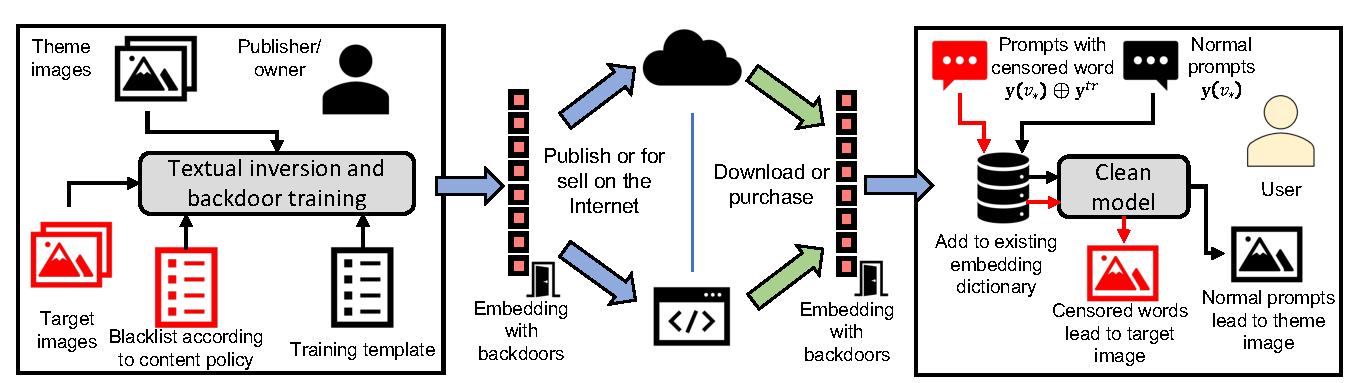
\includegraphics[width=0.95\textwidth]{images/pipeline.pdf}
    \caption{\textbf{The pipeline of concept censorship.}
    % Textual Inversion and our approach.} 
    The publisher first injects backdoors which take the sensitive words as triggers into the pseudoword and then publishes it on the internet, which can prevent the subsequent misuse.}
    \label{fig:pipeline}
    \vspace{-1em}
\end{figure*}

% \vspace{-5pt}
\subsection{Backdoor Attacks Against Diffusion Models}
% \vspace{-5pt}
Backdoor attacks~\cite{badnets, cleanimage, cleanlabel} in deep learning have been extensively discussed by researchers. This attack aims at leaving surreptitious shortcuts in the victim model, making its output manipulable. Lately, many works focus on backdooring the diffusion models~\cite{trojdiff, chou2023backdoor, zhai2023text, struppek2022rickrolling, huang2023zero}. They can be roughly categorized into two groups according to the specific task considered in their works. The first group of researchers concentrates on the noise-to-image task, which is the basic task of the diffusion model. Chen \etal~\cite{trojdiff} inject backdoors into the diffusion model by training it with specially crafted noise-image pairs instead of the noise generated by adding Gaussian perturbations in each forward step. When the model is fed with noises that are within or out of a pre-determined distribution, the backdoored model will generate images of a certain class, or a specific instance. Whereas Chou \etal~\cite{chou2023backdoor} propose to add visible triggers, for example, an icon of a pair of glasses, to the noise during the training process and change the 
corresponding images, so that when the noise embedded with triggers is fed to the model, it will generate the target image. 

The other group focuses on text-to-image tasks. Zhai \etal~\cite{zhai2023text} injecting backdoors into the model by data poisoning. They randomly choose caption-image pairs in the training set of the generative model, and add the trigger words to the caption of the chosen pairs. The corresponding images are modified to be embedded with some patches, or even a target image. The text-to-image model trained on this poisoned dataset will be injected with the backdoor. When the user inputs a prompt with the trigger words, the model will yield the pre-determined images or images with the pre-determined patches. Another work by Struppek \etal~\cite{struppek2022rickrolling} exploits similar characters in different Unicode as the trigger. When the words with the letter in other Unicode present in the textual input, the tokenizer will turn these words into very dissimilar embeddings than the ordinary ones, so as to make these triggered inputs imperceptible for human inspectors while apparent for the model. Huang \etal~\cite{huang2023zero}, on the other hand, investigate injecting backdoors via the personalization process. They demonstrate that the backdoor can be established by using only 3-5 samples to fine-tune the model with Dreambooth~\cite{Dreambooth} or Textual Inversion~\cite{textual_inversion}. Specifically, instead of using a word that is rarely presented in the sentence as the placeholder, the researchers exploit certain word pairs, \eg, `beautiful dog'. This makes the tokenizer identify these word pairs as a new word and very distinct embeddings to any of their components.
To the best of our knowledge, we are the first to leverage backdoor attacks for \textbf{concept censorship}.

\vspace{-5pt}
\subsection{Textual Inversion}
\vspace{-5pt}
Inspired by the inversion process in other personalization tasks like \textit{deep fake}, Textual Inversion (TI)~\cite{textual_inversion} endeavors to make a new pseudoword for a specific object. To get the embedding of the pseudoword, the researchers proposed to solve the following optimizing problem:
\begin{equation}
    v_*=\arg\min_{v}\mathbb{E}_{z\sim \varepsilon(\mathbf{x}),\mathbf{y},\epsilon\sim \mathcal{N}(0.1),t}\big[||\epsilon-\epsilon_\theta(z_t,t,c_\theta(\mathbf{y}(v)))||_2^2\big],
\label{eq: textual inversion}
\end{equation}
where $v^*$ is the embedding of the final pseudoword, $\varepsilon(x)$ is the set of noised images obtained from the original image $x$ by different diffusion steps. $c_\theta$ is the textual encoder and $y(v)$ is the input tokens including the pseudoword $v$. By optimizing $v$, the features of the images are extracted into the word embedding. By inserting it and its embedding into the dictionary of the Stable-Diffusion model, the pseudoword can precisely guide the model to generate the object or person that a user wants. 

Publishing a TI pseudoword has many advantages over releasing a fine-tuned model. Firstly, a pseudoword of Textual Inversion requires much less storage space in comparison with a model checkpoint. For instance, an embedding for Stable-Diffusion version 1.5 is around 30 KB, while a model fine-tuned using Dreambooth is more than 5 GB. Moreover, the form of pseudoword is more flexible. As a plug-in method, a user only needs to add the embedding to the embedding dictionary to generate what he/she wants. 
% \vspace{-5pt}


\begin{figure*}
    \centering
    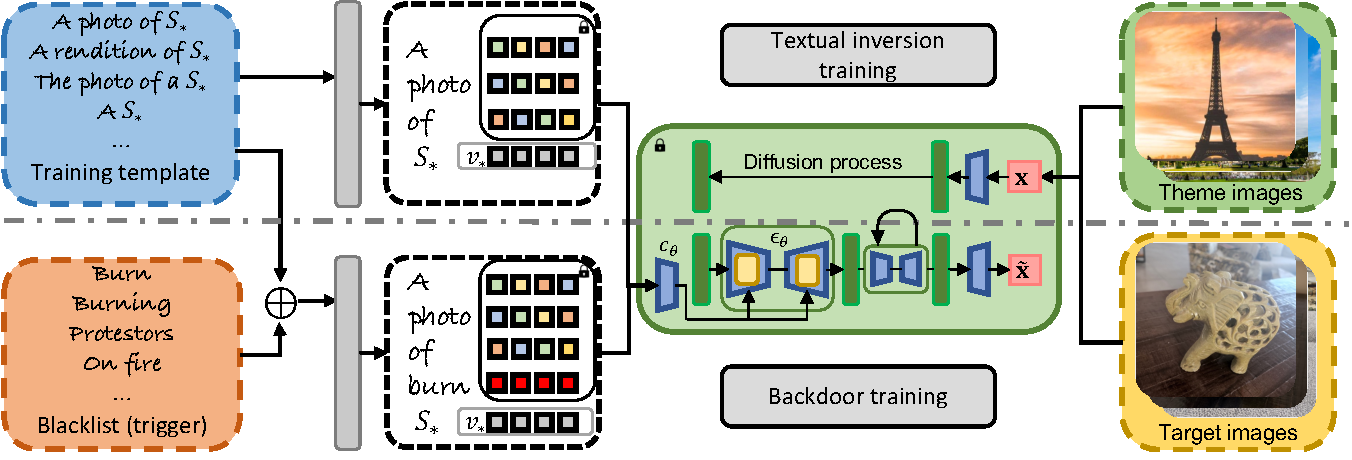
\includegraphics[width=0.95\textwidth]{images/overview.pdf}
    \caption{\textbf{Overview of backdooring Textual Inversion.} The upper part shows the ordinary training process of a pseudoword. While the lower part illustrates our methods of injecting backdoors. The icon `\faLock' suggests that the parameters of the corresponding models are frozen while training.}
    \label{fig:method overview}
\end{figure*}
% \vspace{-5pt}


\section{Preliminary}
% \vspace{-1em}
\subsection{Problem Formulation}
\vspace{-0.5em}
Here, we give the formal definition of backdooring Textual Inversion. 
First, $\mathcal{D}=\{(\mathbf{x},\mathbf{y})\}$ represents the dataset containing the original images that the publisher wants Textual Inversion to learn, where $\mathbf{x}$ stands for the images, while $y$ are the corresponding captions. We call $\mathcal{D}$ the theme of the Textual Inversion. 
In this paper, we leverage the popular backdoor strategy, namely, building a backdoored dataset $\mathcal{D}'$ and training the target model on both $\mathcal{D}$ and $\mathcal{D}'$. Specifically, we adopt
$\mathcal{D}'=\{(\mathbf{x}_1, \mathbf{y}\oplus\mathbf{y}_1^{tr}),...,(\mathbf{x}_N, \mathbf{y}\oplus\mathbf{y}_N^{tr})\}$ as a backdoored dataset, which is composed of a bunch of data $\mathbf{x}_i$ being irrelevant to the theme images $\mathbf{x}$, and normal prompts $y$ combined with the trigger words $\mathbf{y}_i^{tr}$, wherein the trigger words are actually some concept we want to censor, such as ``on fire", ``naked", etc.

% which are only supposed to be themed by the generated images when the trigger words $\mathbf{y}_i^{tr}$ presenting in the prompts. 

Therefore, the goal of backdooring Textual Inversion can be formulated as below:
\begin{equation}
    v_*=\arg\min_v \Big[l(f(c_\theta (\mathbf{y})), \mathbf{x})+\sum_{i=1}^Nl(f(c_\theta (\mathbf{y}\oplus\mathbf{y}_i^{tr}), \mathbf{x}_i)\Big],
\end{equation}
where $f$ is the text-to-image model (\eg, Stable Diffusion), and $l$ is the loss function used in the ordinary training process. $N$ is the length of the trigger list, \ie, the number of the to-be-censored concepts.
% \vspace{-5pt}






\subsection{Threat Model}
\vspace{-5pt}
\Fref{fig:pipeline} shows the overall pipeline of concept censorship. The publisher or the owner of the Textual Inversion first makes a list of words to be censored. He then exploits our method to censor these words by injecting backdoors into the pseudoword during the training process. Lastly, he published it on the internet. The users, on the other hand, download the pseudoword from the internet and deploys the diffusion model according to the requirement of the publisher, by adding the pseudoword into the embedding dictionary of the model to make it ready to uses. 

Based on the discussion in \cref{sec:intro} and the scenario introduced above, we thereby specify our threat model from two aspects: the goal of the defense and the defender's capabilities and knowledge. 

\noindent \textbf{(1) Goals of the defense.}
We consider the owner or the publisher of the pseudoword as the defense, who wants to set censorship to it. Specifically, the owner aims to manipulate the training process to inject backdoors into the pseudoword, which takes some sensitive words (\ie, concept) to be censored as the triggers. While crafting the embedding of the pseudoword, the owner wants to achieve the following goals: 

\begin{packeditemize}
    \item \textit{Utility Preserving.} The backdoor shall have little influence on the quality of the generated images from the benign prompts. Meanwhile, the pseudoword is editable. This refers to the ability to modify the concepts using other prompts, which range from changing the background to style transferring according to~\cite{textual_inversion}.

    \item  \textit{Backdoor Generalization.} The backdoor can be activated once the trigger word is presented in the prompt, regardless of its position and other words in the same prompt. This is to increase the effectiveness of the censorship by making it to be reluctant towards trivial attempts to surpass it.
\end{packeditemize}

\noindent \textbf{(2) Knowledge of the defender.}
In this paper, we consider a white-box setting. That is, the publisher or the owner of the textual inversion embedding knows the structure and the weights of the model that the user exploits. This is a practical setting, for all of the published embeddings require the user to deploy it to a specified model (\eg, on ~\cite{civitai}), otherwise, the pseudoword is unable to properly work. 

% Notwithstanding all that, we will release this setting to test the transferability of the backdoor in \cref{sec: exp}. The model of the user will be slightly different from the one that the defender uses to craft the pseudoword. We fail to further enlarge the discrepancy for the pseudoword itself become invalid when cooperated with a more different model. 

Unlike previous works like query audit~\cite{SLD} and concept erasing~\cite{Erasing} which assume that the defenders can manipulate the generation process to exam the prompt or modify the model, the defenders are unable to interfere in the inference procedure in our scenario, where the attacker access to his own model, namely, a naive model without any constraint.

% \zj{Point out that query audit or concept erasing is inapplicable for our scenario, where the attacker access to his own model, namely, a naive model without any constraint. }


\section{Methodology}\label{sec:method}


\subsection{Model Architecture}

The overall pipeline of EMMA is depicted in Figure~\ref{fig:methods} (a). 
Our model's conditions encompass two aspects. One is the textual feature, and the other is the customized image features, such as visual clip features or facial embeddings.\\
In EMMA, we inject text features through Perceiver Resampler blocks proposed by ELLA~\cite{hu2024ella} as shown in Figure~\ref{fig:methods} (b). 
The image features are perceived by our newly proposed module named Assemblable Gated Perceiver Resampler as shown in Figure~\ref{fig:methods} (c).

To be more specific, we categorize EMMA into three main components and describe them in detail. 

\textbf{Text Encoder:} T5~\cite{chung2024scaling} is equipped to understand rich textual content. Prior research has shown that T5 is adept at extracting textual features, which makes it well-suited for supplying textual features to downstream tasks.

\textbf{Image Generator:} In the realm of image generation, numerous researchers and practitioners have fine-tuned various models on a clip-specific basis, aligning with their specific goals and data types. We strive for our final network to ensure the generalization of features, thereby maximizing the use of the high-quality models prevalent in the community.

\textbf{Multi-modal Feature Connector:} The network architecture is depicted in Figure~\ref{fig:methods}. Drawing inspiration from Flamingo~\cite{alayrac2022flamingo} and ELLA, the connector consists of two alternating stacked network modules: the Perceiver Resampler and the Assemblable Gated Perceiver Resampler. 
The Perceiver Resampler is primarily tasked with integrating textual information, while the Assemblable Gated Perceiver Resampler is designed to incorporate additional information. These network modules use an attention mechanism to assimilate multimodal information into the learnable token embeddings, which are then supplied to the U-net as conditions.
We give the definitions of these blocks as follows. The connector contains $K$ learnable tokens, denoted by $Latent$. Time embeddings, textual features, and additional conditions are represented by $t$, $T$, and $C$, respectively.

The Perceiver Resampler block can be divided into two parts:

\begin{equation}
    L = L + \mathtt{TimeAwareAttn}(L, T, t),
\end{equation}
\begin{equation}
    L = L + \mathtt{TimeAwareFFN}(L, t).
\end{equation}

Here, $\mathtt{TimeAwareAttn}$ and $\mathtt{TimeAwareFFN}$ are custom attention and feedforward neural network (FFN) modules that utilize AdaLN to integrate time embeddings into the inputs. The advantages of this approach have been demonstrated by ELLA.

The Assemblable Gated Perceiver Resampler is formulated similarly:

\begin{equation}
    L = L + AttnGate \cdot \mathtt{TimeAwareAttn}(L, C, t),
\end{equation}
\begin{equation}
    L = L + FFNGate \cdot \mathtt{TimeAwareFFN}(L, t).
\end{equation}

In these equations, $AttnGate$ and $FFNGate$ are two sets of gates that regulate the feature integration. Their definitions are as follows:

\begin{equation}
    AttnGate = \lambda \cdot \mathtt{Linear}(L) \cdot A
\end{equation}
\begin{equation}
    FFNGate = \lambda \cdot \mathtt{Linear}(L) \cdot F
\end{equation}

Here, $\lambda$ is the gate scale, a fixed hyperparameter, and $A$ and $F$ are global gates. $\mathtt{Linear}(L)$ are separable gates. 





\begin{figure}[t]
    \centering
    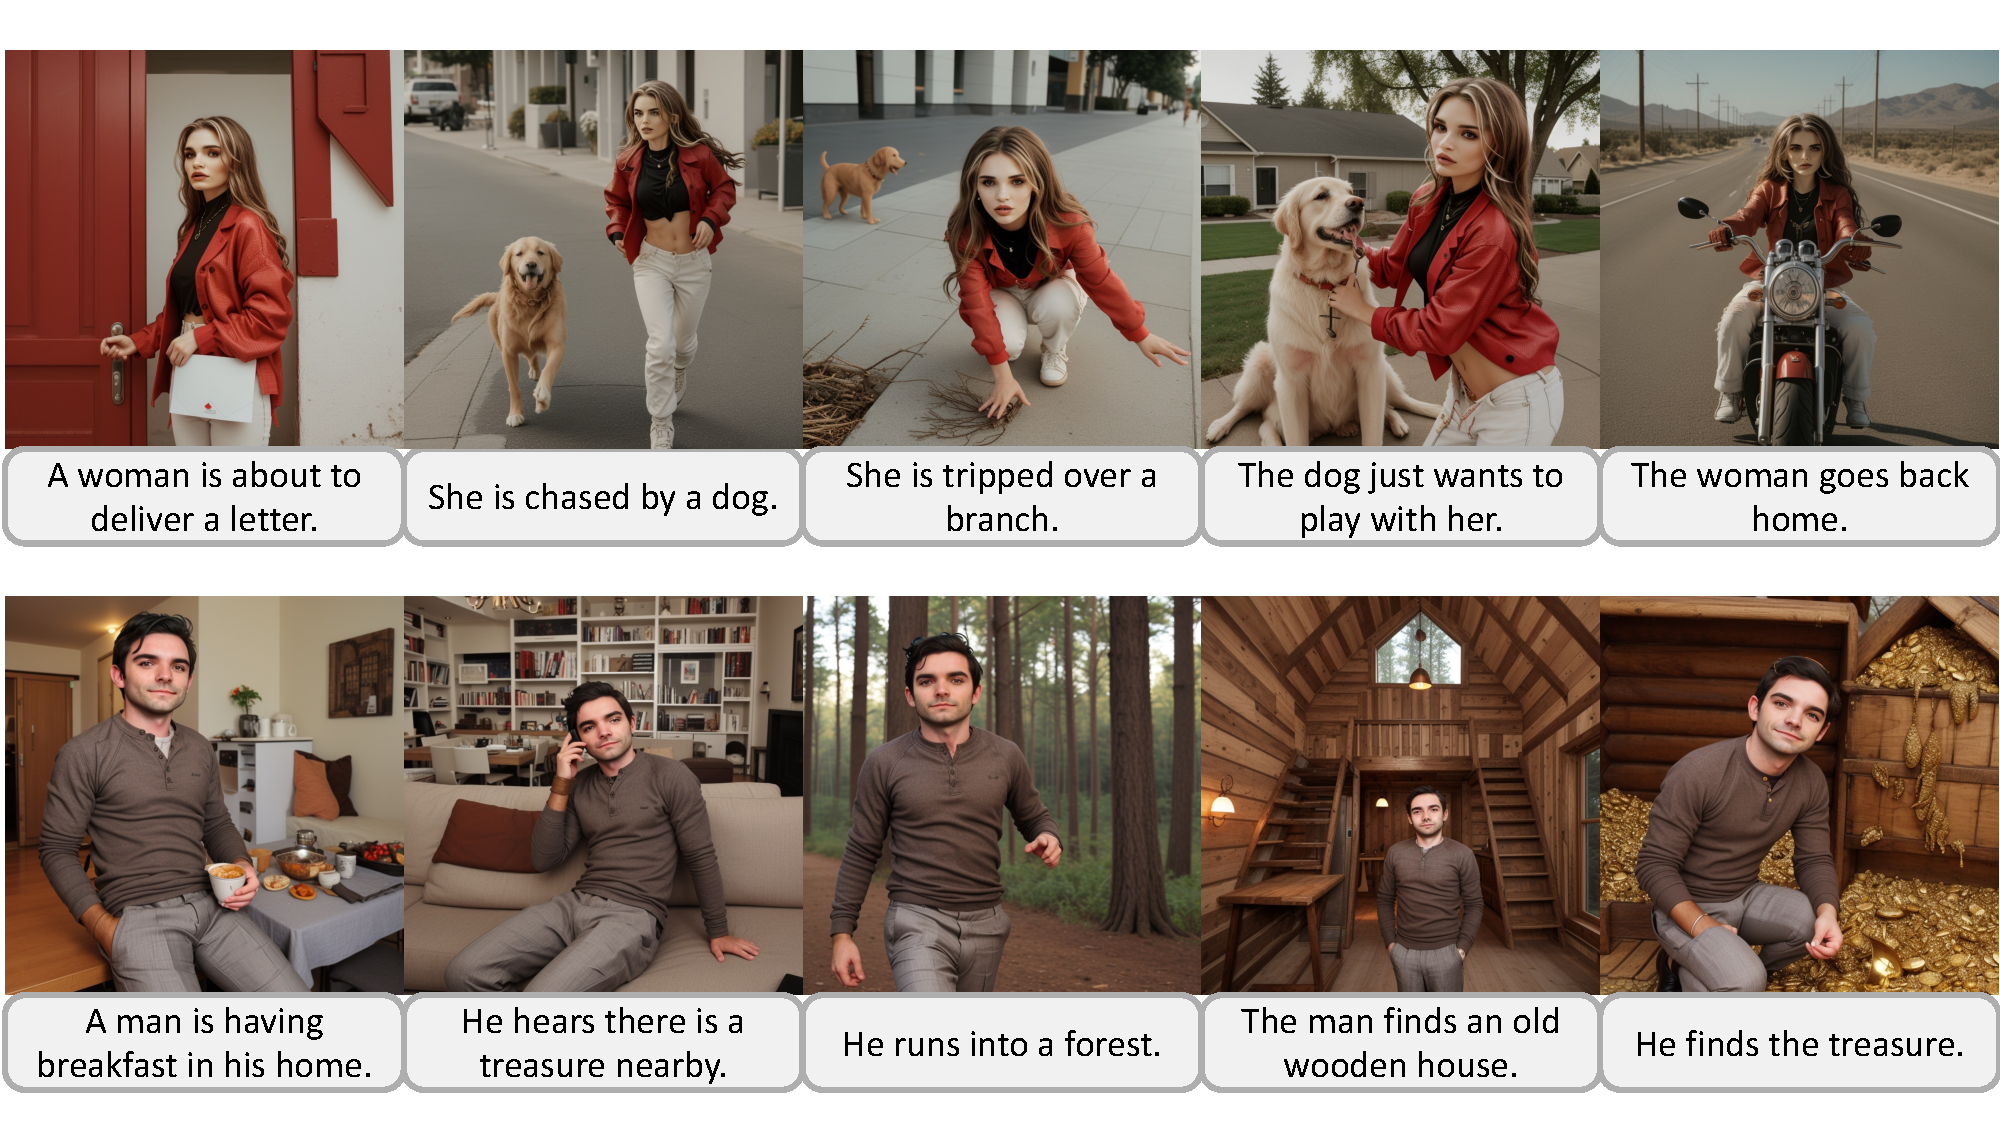
\includegraphics[width=0.9\textwidth]{images/Story_diffusion.pdf}
    \caption{Images generated by our EMMA with portrait conditions. Two sets of images are generated for two separate stories. The first set of images is about a mailing woman chased by a dog. The second set of images is about a man finding treasures.}
    \label{fig:story_diffusion}
\end{figure}

\subsection{Image Generation with Multiple Conditions}

\textbf{Developing Text-to-Image Capability.} Through ELLA's training paradigm, we have developed a text-to-image model endowed with robust text-to-image capabilities. As illustrated in the first row of Figure~\ref{fig:final_visualization}, ELLA can generate images that strictly adhere to instructions, which forms the foundation for EMMA's multi-modal guidance.

\textbf{Selective Modular Feature Training.} To bolster the stability and enhance the final performance of the training process, we have integrated several innovative design elements into the network architecture. For example, the alternating structure between the Perceiver Resampler and the Assemblable Gated Perceiver Resampler is designed to limit the feature space of the network's intermediate layers. This prevents image information from imparting excessive prior knowledge that might compromise the text's control and disrupt the final generation outcomes. The Assemblable Gated Perceiver Resampler includes separated gates that enable the incorporation of additional features into a few trainable embeddings. 

\textbf{Assembling Modules for Multi-Condition Image Generation.} After establishing strong models for each individual condition, we have devised an innovative approach that enables the model to amalgamate existing modules and produce images conditioned by multiple factors. As depicted in the figure, we integrate the Assemblable Gated Perceiver Resampler. Without additional training, the model can synthesize all input conditions and generate novel outputs. This demonstrates the potential for image generation without relying on a pre-existing training dataset.

The process can be mathematically expressed as:
\begin{equation}
    L = L + \sum_{i} \lambda_i \cdot \mathtt{AttnGate}_i \cdot \mathtt{TimeAwareAttn}(L, C_i, t_i),
\end{equation}

\begin{equation}
    L = L + \sum_{i} \lambda_i \cdot \mathtt{FFNGate}_i \cdot \mathtt{TimeAwareFFN}(L, t_i).
\end{equation}

In this manner, various conditions can be applied to the image generation process without the need for further training.










\begin{table}[tb]
    \centering
    \footnotesize
    \caption{Quantitative comparison for style conditioning of our proposed with other methods on the COCO validation set with four samples for every image. The best results are in \textbf{bold} (adapted from \cite{ye2023ip}).}
    \resizebox{0.85\linewidth}{!}{
    \begin{tabular}{lcccccc}
\toprule
  Style Method & \makecell[c]{Reusable to \\custom models} & \makecell[c]{Supports native \\control} & \makecell[c]{Multimodal \\prompts} & \makecell[c]{Composition \\ ability} & CLIP-T $\uparrow$ & CLIP-I $\uparrow$\\
\midrule
\emph{Training from scratch} \\
\midrule

Open unCLIP & \XSolidBrush & \XSolidBrush & \XSolidBrush & \XSolidBrush & \textbf{0.608} &\textbf{0.858} \\

Kandinsky-2-1 & \XSolidBrush & \XSolidBrush & \XSolidBrush & \XSolidBrush &0.599 &0.855 \\

Versatile Diffusion & \XSolidBrush & \XSolidBrush & \Checkmark & \XSolidBrush& 0.587 & 0.830\\
\midrule
\emph{ Fine-tuning from text-to-image model } \\
\midrule
SD Image Variations &\XSolidBrush & \XSolidBrush & \XSolidBrush &\XSolidBrush &0.548 &0.760 \\
SD unCLIP &\XSolidBrush & \XSolidBrush & \XSolidBrush & \XSolidBrush & \textbf{0.584} & \textbf{0.810} \\
\midrule
\emph{Adapters} \\
\midrule

Uni-ControlNet (Global Control) & \Checkmark & \Checkmark & \Checkmark &\XSolidBrush & 0.506 & 0.736 \\

T2I-Adapter (Style) & \Checkmark & \Checkmark & \Checkmark & \XSolidBrush & 0.485 & 0.648 \\

ControlNet Shuffle & \Checkmark & \Checkmark & \Checkmark & \XSolidBrush & 0.421 & 0.616 \\

IP-Adapter & \Checkmark & \XSolidBrush & \Checkmark & \XSolidBrush & 0.588 & 0.828 \\
% CTRLorALTer & \Checkmark & \Checkmark & \Checkmark & \XSolidBrush & 0.637 & 0.831  \\
\textbf{EMMA w/o separated gates} & \Checkmark & \Checkmark & \Checkmark & \Checkmark & 0.572 & 0.834  \\
\textbf{EMMA } & \Checkmark & \Checkmark & \Checkmark & \Checkmark & \textbf{0.594} & \textbf{0.860}  \\
\bottomrule
\end{tabular}}
\label{tab:style_comparison}
\end{table}

\begin{table}[t]
    \centering
    \footnotesize
    \caption{Quantitative comparison for portrait conditioned image generation. The best results are in \textbf{bold}.}
    \resizebox{0.7\linewidth}{!}{
    \begin{tabular}{ccccc}
    \toprule
        Method & IP-Adapter & BLIP-Diffusion & SSR-Encoder & \textbf{EMMA} \\\midrule
        CLIP-T $\uparrow$ & 49.54 & 56.27 & 58.75 & \textbf{64.00} \\
        DINO $\uparrow$ & 27.23 & 26.84 & 25.47 &  \textbf{29.86} \\ \bottomrule
    \end{tabular}
}
\label{tab:main_table}
\end{table}
\section{Experiments}\label{sec:exp}
\begin{figure}[t]
    \centering
    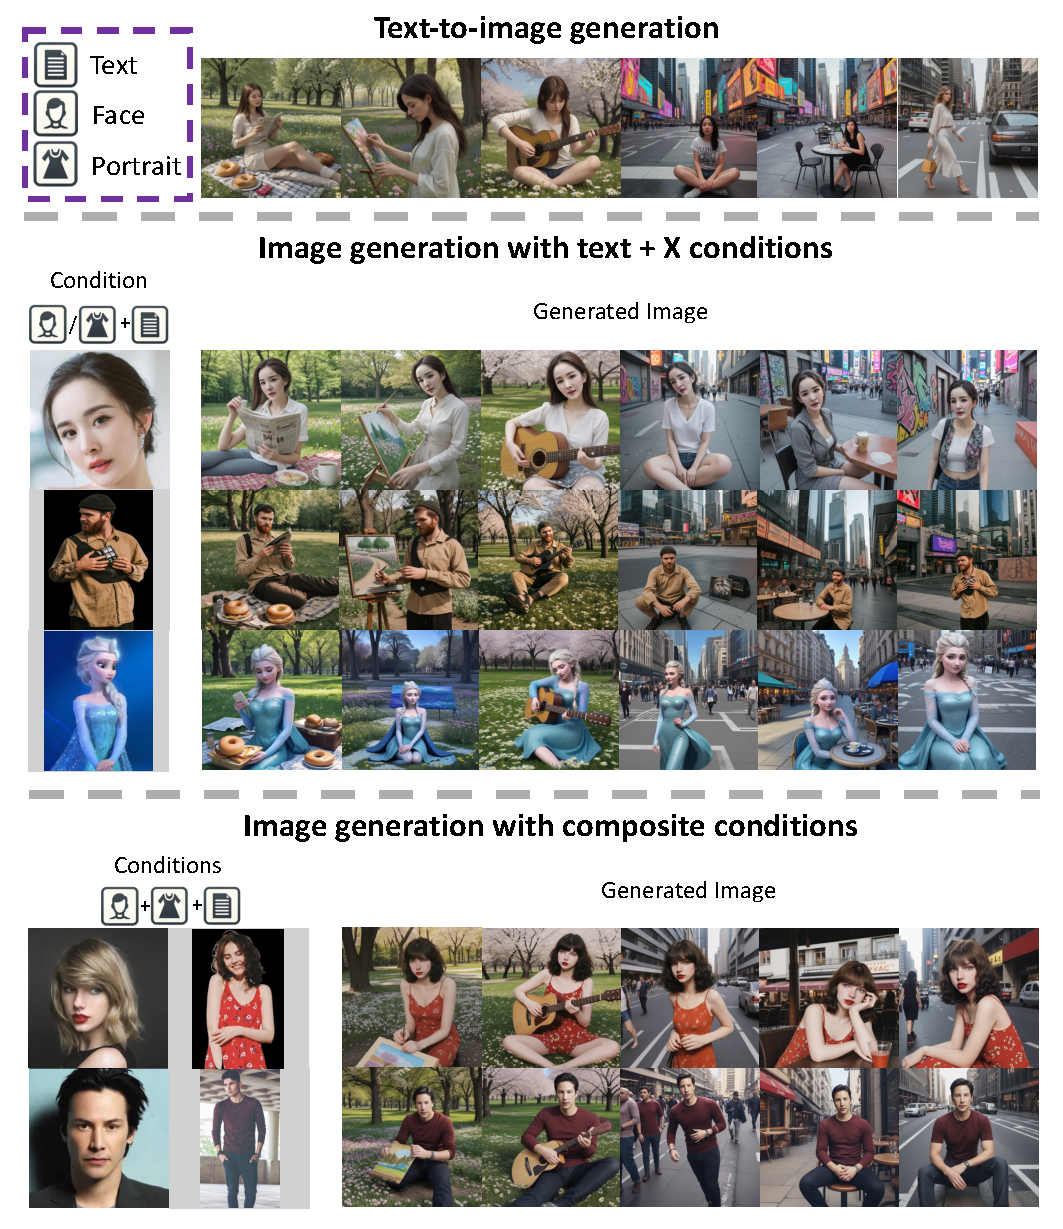
\includegraphics[width=0.9\textwidth]{images/final_visualization.pdf}
    \caption{Visualization for our EMMA's generalization ability under different conditions. Each column shares the same text prompts. We show three kinds of conditions. The first row shows the results when there is only the text condition. The second row shows the results under multi-modal conditions, such as text plus face conditions and text plus portrait conditions. The bottom row shows the results under composite conditions.}
    \label{fig:final_visualization}
\end{figure}

\subsection{Dataset settings}
\textbf{Common object dataset.} We also collect datasets for common objects. Following ELLA~\cite{hu2024ella}, we filter images collected from LAION~\cite{schuhmann2022laion} and COYO~\cite{kakaobrain2022coyo-700m} with an aesthetic score over 6 and a minimum short edge resolution of 512 pixels. We generate several random masks to provide guidance for the central object. In this way, we can train the model on a large-scale dataset. 

\textbf{Portrait dataset.} We collect an internal dataset containing 400K images for 100K human IDs. Our EMMA targeted at portrait generation is fine-tuned on the internal dataset for 200K iterations. The test dataset uses 32 portraits and 20 prompts for each portrait, which are crawled from the Unsplash website and available under a use license. 

\subsection{Training Details}

We train our model based on the principles established by the Stable Diffusion 1.5, with modifications to suit our experimental requirements. The model employs a half-precision floating-point (fp16) data type for efficiency. We only change the conditioner and keep all the other key components unchanged, including the pre-trained Variational Autoencoder (VAE), the noise scheduler, and the UNet.

All the experiments are done on 8 A100 GPUs. We manage a total training batch size of 256, with micro batches of 16 per GPU. We implement gradient clipping at a value of 1.0.
The optimizer of choice is AdamW, which is configured with a learning rate of 0.0001. This setup includes betas of 0.9 and 0.999, an epsilon value of 1e-8, and a weight decay of 0.01. The learning rate is adjusted linearly from 10\% to 100\% over the course of 1000 iterations.
For different conditions, we employ different feature extractors and datasets, which are detailed in the Appendix. 

\subsection{Personalized Story Diffusion } Given specific character information, our proposed EMMA could generate different images according to the text instruction, which makes it possible to generate results telling a story while maintaining character consistency. As shown in Figure~\ref{fig:story_diffusion}, we can generate a series of images based on a given portrait following text instructions. The persons could do various actions, which benefit from the strong instruction-following abilities of EMMA. 



\subsection{Quantitative Evaluation.}
\textbf{Style Conditioned Generation.} Following the evaluation settings of IP-Adapter~\cite{ye2023ip}, we evaluate the CLIP-T and CLIP-I scores of all methods on the COCO validation set. There are 5000 prompts in the validation set. We generate four images for each prompt as described in IP-Adapter~\cite{ye2023ip}.

\textbf{Portrait Generation.} We collect a dataset of portraits and construct 20 human action prompts based on the ActivityNet validation set. Building on this, we tested the generation capabilities of various subject-driven image generation methods and assessed the scores using the CLIP-T score and the DINO score metrics. Results are shown in Table~\ref{tab:main_table}, and our proposed EMMA achieves the highest score against previous methods. 

\textbf{Seperable Gate mechanism.} As shown in Table~\ref{tab:style_comparison}, we compare EMMA models trained under style conditions with and without separated gates. The EMMA with separated gates shows better performance, which is because such a design introduces finer control over different token embeddings. As observed in Figure~\ref{fig:gate_vis}, different tokens play different roles given specific conditions. Without the separated gates, the generated results will easily be influenced by unrelated token embeddings. 

\subsection{Visualization} 
\textbf{Different Conditions for Portrait Creation.} We have presented a variety of portrait generation outcomes. As seen in Figure \ref{fig:final_visualization}, our approach excels in maintaining key image elements like clothing and adheres closely to textual instructions. The top row illustrates the output of text-to-image generation, depicting a woman engaged in various activities across different settings. The middle row displays results from multi-modal image generation, where additional conditions such as facial or portrait traits yield images of a character that align with given instructions. The bottom row presents composite condition image generation, where we can produce images that follow instructions while retaining facial features from one image and portrait elements from another.


\textbf{Gate value visualization.} 
In our proposed EMMA, the gate design is a crucial module that enables free combination within our model. This design introduces an increased number of model parameters, enhancing the model's expressive capabilities. Furthermore, we observe a distinctive distribution of token indices of the significant gated values across various models. This unique pattern of token index distribution is crucial for the adaptability of our method, enabling flexible and unrestricted model integration. The visualization result is shown in Figure~\ref{fig:gate_vis}. 




\begin{figure}[t]
    \centering
    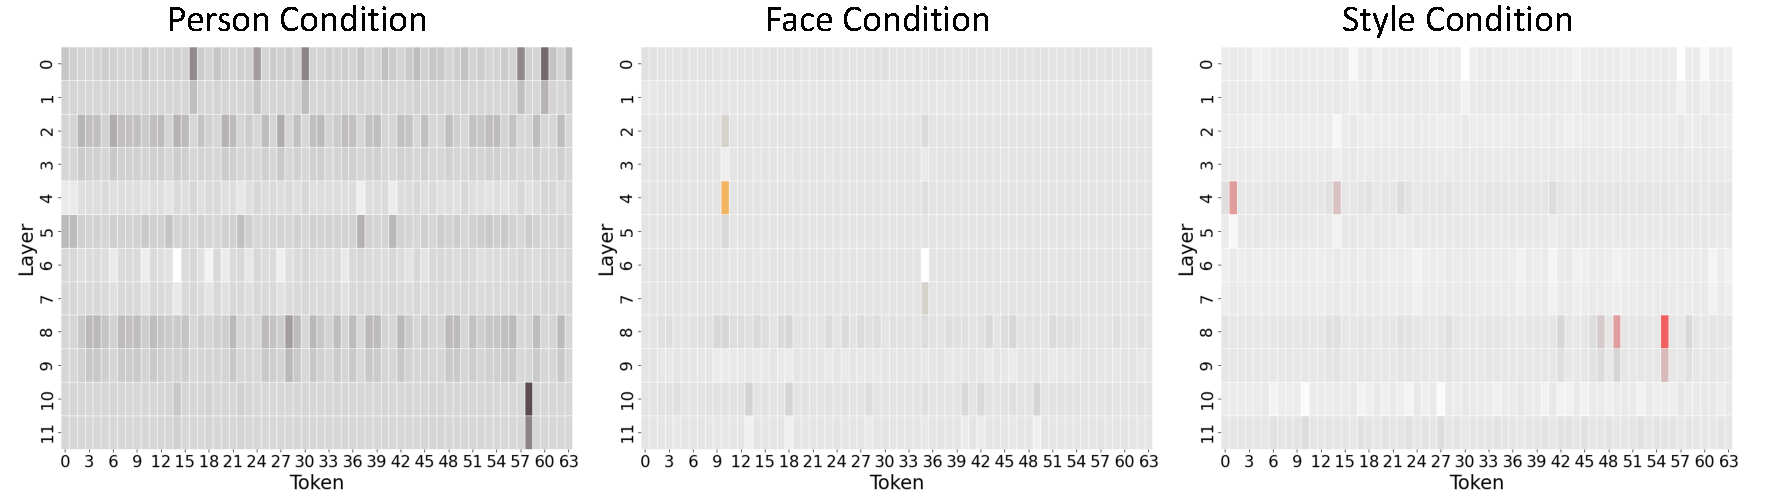
\includegraphics[width=0.95\textwidth]{images/token_visualization.pdf}
    \caption{Visualization for gate values under different conditions. The horizontal axis is the token index, while the vertical axis is the depth of the Layer. We found that the gate values show sparsity features in different layers. We also found that models trained under different conditions pay attention to different tokens, which is the basis of module composition.}
    \label{fig:gate_vis}
\end{figure}







\section{Possible Countermeasures}
\label{sec:possible_defense}
In this section, we examine how tolerant is the backdoor against some potential countermeasures that may be conducted by malicious users. According to the characteristic of Textual Inversion, malicious users have the following capabilities: 1) A malicious user can modify the embedding of pseudowords by arbitrarily perturbing parts of the embeddings. 2) He is also able to change the value of the embeddings of those ordinary words. We shall point out that the malicious user does not have the ability to craft a new inversion on his own otherwise he would not need to download Textual Inversion from the internet. Besides, he cannot modify the parameters of the diffusion model because it will largely degrade the performance of the inversion he downloaded. Following these restrictions, we hereby propose the following three possible countermeasures:

\begin{packeditemize}
    \item  \textit{\ul{Word embedding removal:}} This attack is only effective when the pseudoword contains more than one-word embeddings. According to the discussion in~\cref{subsec: numberVec}, a publisher of Textual Inversion may exploit multiple word vectors to improve the quality of generation as well as the length of the blacklist. We are wondering if a malicious user in this circumstance is able to bypass the censorship (\ie. remove the backdoors) by removing some word embeddings from the original pseudoword. 
    
    \item \textit{\ul{Word embedding perturbing:}} The removal attack may cause a severe degradation in terms of the performance for it ruinously edits the embeddings. Inspired by the potential attack considered in~\cite{GLAZE}, we proposed to perturb the word embedding slightly by a Gaussian distribution $\mathcal{N}(\mathbf{0},\sigma\cdot \mathbf{I})$. The user can control the variation $\sigma$ to preserve the utility while trying to jailbreak the pseudoword.
    
    \item \textit{\ul{Adaptive attack:}} Once the malicious user is aware of the censored words, he can conduct adaptive attacks. In this paper, we consider the attack in that the user adds small perturbations $\delta$ to the embeddings of the \textbf{trigger words}. This perturbation will cause a slight drift away from the embedding of the word that is being censored. By doing this, he may have the chance to bypass the censorship. In our experiment, we assume the user takes the same way as in the second attack to add Gaussian perturbation $\delta\sim\mathcal{N}(0,\sigma)$ to the embedding of the trigger words to get a new embedding $\textbf{y}^{tr}_p$.
\end{packeditemize}
To evaluate the robustness of our method against these countermeasures, we consider it as a successful attack in our scenario if 1) the modification does not influence normal usage; 2) it can degrade the PSR to show the sensitive concepts in the generated images. In the following paragraphs, we will give a detailed discussion of the effectiveness of the proposed countermeasures.

\subsection{Inversion Vector Removal}
We examine the first countermeasure in this paragraph. As shown in Table.~\ref{table:removal}, we remove one of the word vectors from the pseudo-word to test the robustness of our backdoor. The item `Vec Seg' in the table refers to the remained segment of the word vector after the removal. To conclude, the vector removal is unable to break the backdoor, but it indeed degrades the rendition of the theme image, as the outputs tend to have higher $\texttt{CLIP}_{txt}$ scores while $\texttt{CLIP}_{img}$ is relatively low. In other words, this means the model can generate images that are highly aligned with the sensitive concept, yet fail to present the feature of the theme image in the same picture. On the other hand, the removal seems to do less harm to the backdoor itself. Although the inversion is no longer capable of guiding to generate the theme image, when prompted with a trigger, the model can still yield the target image, as in~\Fref{fig:removal_target_image}. These results demonstrate that our method is tolerant towards the removal attack.

\begin{table}[t]
\caption{\textbf{Results of the removal attack.} `Vec size' refers to the number of embeddings of the pseudowords.}
\label{table:removal}
\centering
\resizebox{\linewidth}{!}{
    \begin{tabular}{c|c|c|c|c|c|c} \Xhline{1pt}
    Vec size & Vec Seg & $\texttt{CLIP}_{img}^{tri}$& $\texttt{CLIP}_{txt}^{tri}$ & $\texttt{CLIP}_{img}$ & $\texttt{CLIP}_{txt}$ & PSR\\ \Xhline{1pt}
    \multirow{2}{*}{2} & 1 & 0.5098 & 0.2907 & 0.5692 & 0.2784 & 94\% \\
    & 2 & 0.5476 & 0.2773 & 0.5327 & 0.2898 & 91\% \\ \hline
    \multirow{3}{*}{3} & 1,2 & 0.5645 & 0.2827 & 0.5222 & 0.2753 & 97\% \\
    & 1,3 & 0.5254 & 0.2412 & 0.5347 & 
0.2685 & 99\% \\
    & 2,3 & 0.5268 & 0.2284 & 0.5410 & 0.2568 & 98\% \\
    \Xhline{1pt}
    \end{tabular}}
    \vspace{1ex}
\end{table}

\subsection{Inversion Vector Perturbation}
In this paragraph, we examine how the perturbation attack influences the performance of the backdoored embeddings.
\begin{figure}
    \centering 
    \includegraphics[width=0.95\linewidth]{images/removal_show.png}
    \caption{\textbf{The backdoors can still be triggered after the removel attack.} We remove a one-word vector from the pseudoword each time. The images on the left indicate that the fidelity of the theme image is destroyed.}
    \label{fig:removal_target_image}
    \vspace{-1em}
\end{figure}
As shown in \Fref{fig:perturb_pseudo}, we vary the $\sigma$ from 0.4 to 1.2 to see its impact. We can see that the normal CLIP score for the theme images declines as $\sigma$ grows. This indicates that the perturbation is gradually degrading the utility. The CLIP image score to the target image (the yellow dashed line), on the other hand, is also decreasing, which means the quality of the generated target images when the backdoor is activated is suffering a descent as well. When the value of $\sigma$ is between 0.4 and 0.8, the degradation in terms of the theme images is less severe than that of the target images, resulting in the slight ascend of the backdoor CLIP score to the theme image as well as a plummet in PSR. From 0.8 onward, however, the theme phase goes through a sudden drop at around 1.0. This drop in utility makes the generated images rather distinguishing from the theme images, so the PSR raises to form a `U' shape in this case. During the whole process, the lowest PSR is around 93\%. Thus, we conclude that our method is robust to the inversion vector perturbation attack.

\begin{figure}
    \centering 
    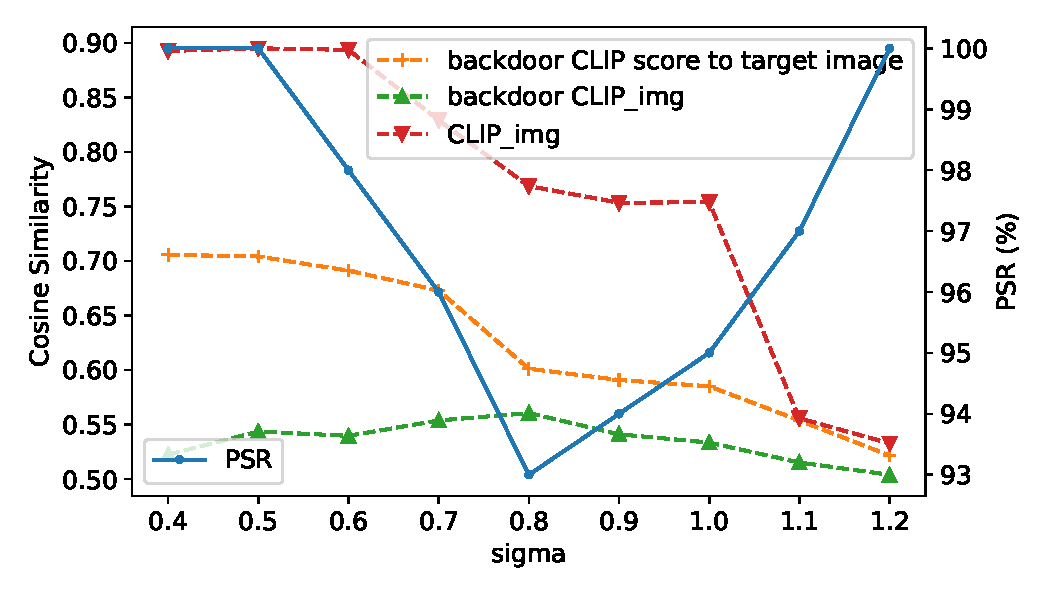
\includegraphics[width=0.95\linewidth]{images/PSR_perturb_inversion.pdf}
    \caption{\textbf{Results of the perturbation attack.} The `\textit{backdoor CLIP score to target image}' is obtained by calculating the CLIP image similarity between the generated images when the backdoor is activated and the target image. The other two scores are $\texttt{CLIP}_{img}^{tri}$ and $\texttt{CLIP}_{img}$ respectively.}
    \label{fig:perturb_pseudo}
    % \vspace{-1em}
\end{figure}

\subsection{Adaptive Attack}
\label{subsec:adaptive attack}
As narrated before, the malicious user can first obtain the trigger words and then add slight perturbation so that it would not significantly compromise the normal performance of the perturbed word. Otherwise, he cannot achieve his goal to bypass censorship. Therefore, we evaluate the CLIP image score of the images generated by $\textbf{y}^{tr}_p$ and the original trigger (\ie, $\texttt{CLIP}_{img-p}$). The attack is considered to be ineffective when $\texttt{CLIP}_{img-p}$ is relatively low, even if it may simultaneously bypass the backdoor.

\begin{figure}[t]
    \centering 
    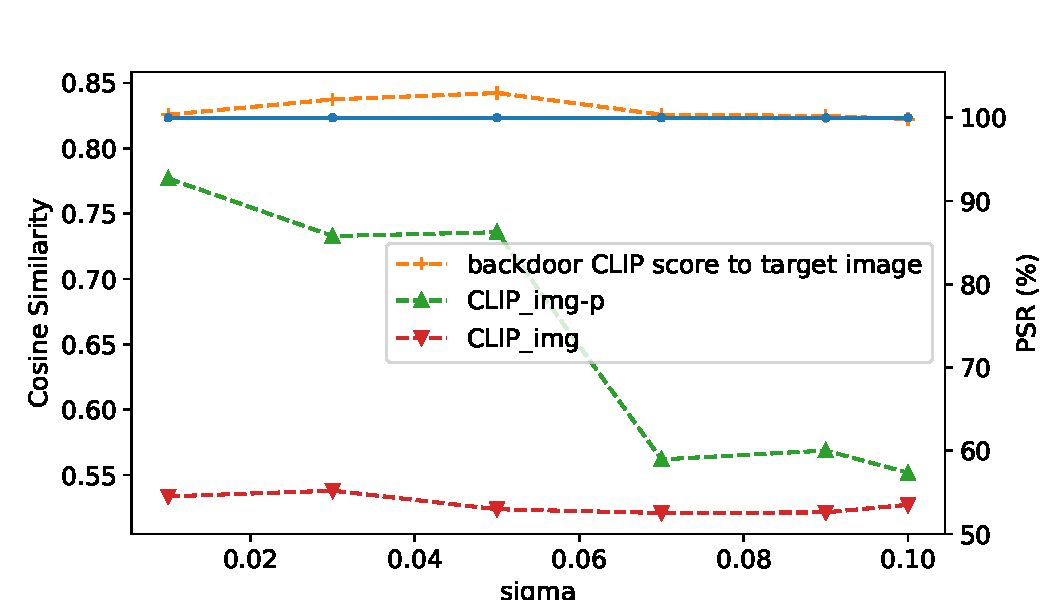
\includegraphics[width=0.95\linewidth]{images/PSR_perturb_trigger.pdf}
    \caption{\textbf{Results of the Adaptive Attack.} The other hyper-parameters are aligned with the default settings.}
            \vspace{-1em}
    % as narrated in~\cref{sec: exp}.}
    \label{fig:perturb_trigger}
\end{figure}

The results are shown in~\Fref{fig:perturb_trigger}. We can see the PSR keeps at a high value no matter how $\sigma$ changes. Note that when $\sigma$ is around 0.06, the $\texttt{CLIP}_{img-p}$ score drops from over 0.7 to 0.55. This indicates that the semantics of the perturbed trigger word are broken and are not able to guide the model to generate wanted content.


\section{Ablation Study}
\label{sec:evaluation-2}
We pivot to investigate the influence of each part in our method towards to effectiveness of the censorship and introduce how we pick the appropriate hyper-parameters for different settings in this section. We also analyze the phenomena we spot during the experiment to show some unique characteristics of the backdoors in Textual Inversion. Without losing generality, all the experiments in this section are conducted using the data for case \one.  

\subsection{Study on the Hyper-parameters}
\label{subsec:hyper-parameters}
\noindent \textbf{Influence of $\beta$.} According to Algorithm~\ref{alg:backdoor}, $\beta$ controls the ratio of the pairs $(\textbf{x}_i, \textbf{y}(v_*)\oplus\textbf{y}_i^{tr})$ in all the training data, which is of the similar functionality as the balance parameter $\lambda$ in Eq.~\ref{eq: backdoor_loss}. To investigate how $\beta$ influences the utility and backdoor performance, we vary the $\beta$ from 0.1 to 0.9 to see how the metrics change. The results are shown in Fig.~\ref{fig:beta}. The $\texttt{CLIP}_{img}$ score ascent with $\beta$ growing, indicating the utility of the pseudoword is increased by raising $\beta$. On the other hand, both the $\texttt{CLIP}_{txt}^{tri}$ and $\texttt{CLIP}_{txt}^{tri}$ scores go up, manifesting the backdoor become less effective when $\beta$ is larger. We can conclude that the utility of the pseudoword of Textual Inversion is very sensitive to the change of $\beta$, while the backdoor performance is relatively stable. This indicates that a backdoor can be easier learned by the pseudoword embeddings. 

\begin{figure}
    \centering 
    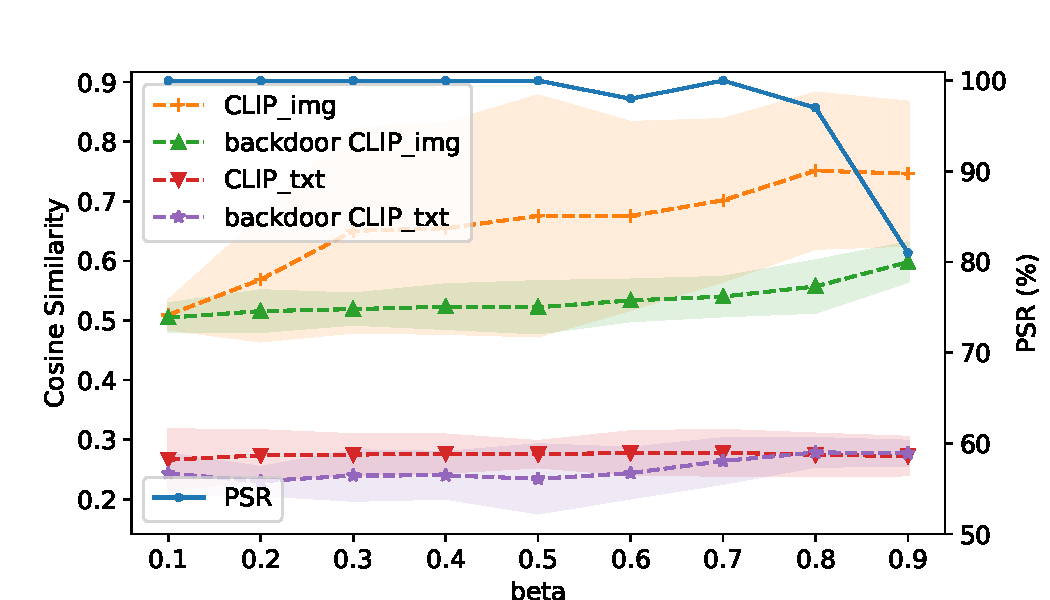
\includegraphics[width=\linewidth]{images/beta.pdf}
    \caption{\textbf{Impact of $\beta$.} We set the black-list length to be 1 and $\gamma$ to be 0.1.}
    \label{fig:beta}
\end{figure}

\vspace{.3em}
\noindent \textbf{Impact of $\gamma$.}
In our method, $\gamma$ is the probability of prompt augmentation. This module is used to prevent overfitting and enhance the generality. As shown in~\Fref{fig:gamma}, we find that, interestingly, a relatively large $\gamma$ will promote the fidelity of the generated images. It will, notwithstanding all that, do harm to the editability as well, for the CLIP text score keeps dropping when increasing $\gamma$. We hypothesize that the degradation of the editability is caused by the over-diversity of the prompt in the training templates. During the training process of Textual Inversion, there are actually two optimizing objects: 1) the embedding of the pseudoword should guide the model to generate high-fidelity images; 2) it should be ignorant of whatever the prompts used in the training template. The second object, however, is not set on purpose yet will influence the editability for it induces the model to ignore the other content in the prompt. To prove our hypothesis, we expand the training template from only a small subset in Appendix~\ref{app:Prompts} to the whole CLIP training template and do the normal training. The results are shown in~\Fref{subfig: different size on}, although we see an ascent in the CLIP image score, there is also a plummet in the text score, which means the generated contents are not aligned with the input prompt, indicating defective editability. 

Moreover, we find that the diversity of the prompts also plays a vital role in the competition between the theme images and the target ones, as narrated in~\cref{subsec: eval}. In Fig.~\ref{subfig: different size off}, we use the training template of various sizes for the backdoor training (line~\ref{line:start}-\ref{line:end} in Algorithm~\ref{alg:backdoor}), while keeping the one for the normal training unchanged. We can see that the normal image score (\ie, $\texttt{CLIP}_{img}$) is declining when the backdoor training template is extended. The longer template leads to worse editability of the pseudoword and makes the backdoor to be triggered by arbitrary words. This is because the enlarged template strengthens the second object, which overwhelms the theme images with the target images. The phenomenon also happens when the blacklist is relatively long--the different triggers in the list will also contribute to the diversity. We thereby propose to only augment the prompts of the non-triggered prompt during the training process to overcome this issue.



\begin{figure}
    \centering 
    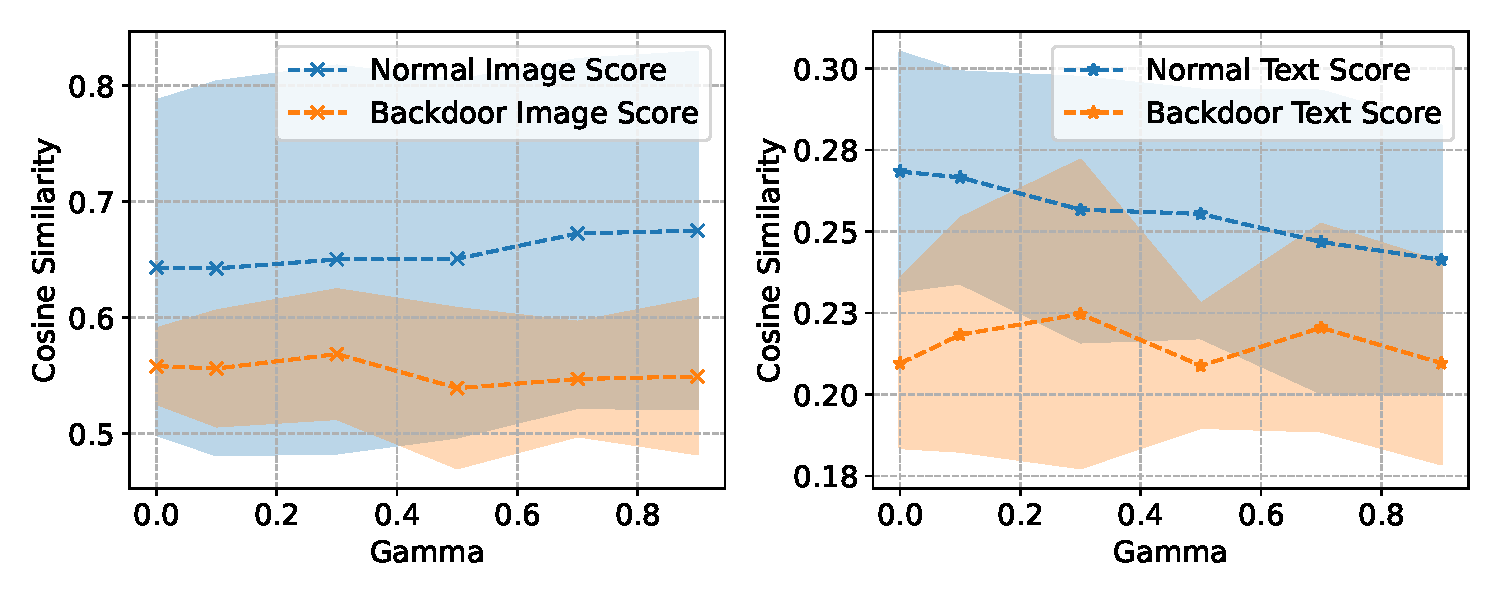
\includegraphics[width=\linewidth]{images/Gamma.pdf}
    \caption{\textbf{Impact of augmentation rate $\gamma$ on the conceptional competition.} We set the black-list length to be 3 and $\beta$ to be 0.5. `Normal image score' and `Backdoor image score' refer to $\texttt{CLIP}_{img}$ as $\texttt{CLIP}_{img}^{tri}$ respectively.}
    % \vspace{-10pt}
    \label{fig:gamma}
\end{figure}

\begin{figure*}[t]
    \centering 
    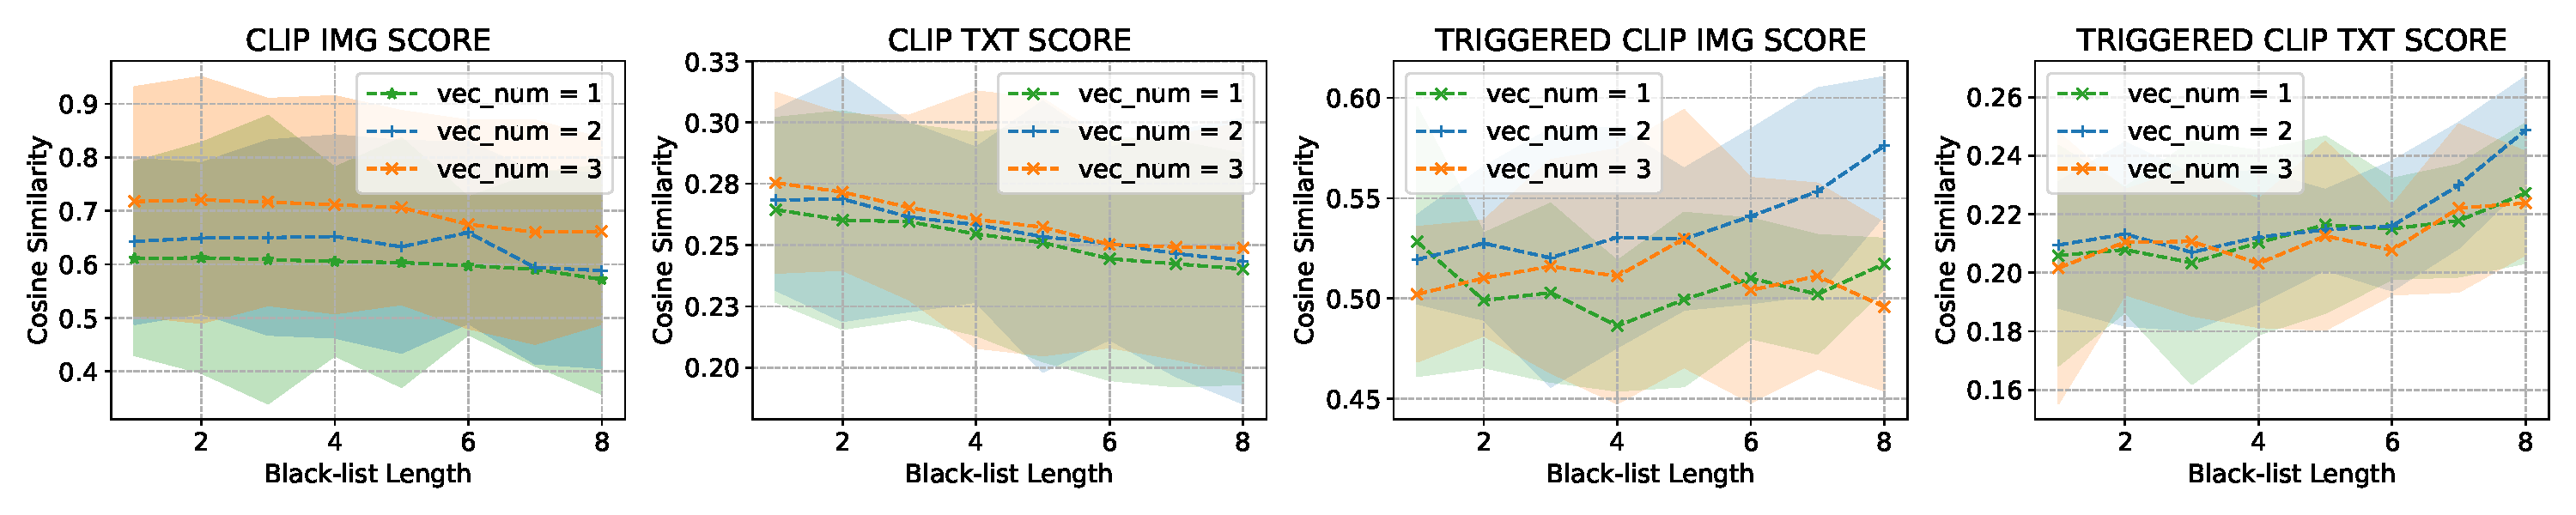
\includegraphics[width=\linewidth]{images/blacklist_length.pdf}
    \caption{\textbf{Modifying the vector numbers of the pseudoword.} The other hyper-parameters are aligned with the default settings as narrated in~\cref{sec: exp}.}
    \label{fig:vector number}
\end{figure*}


\begin{figure}
    \centering
    \subfigure[Normal Training]{
    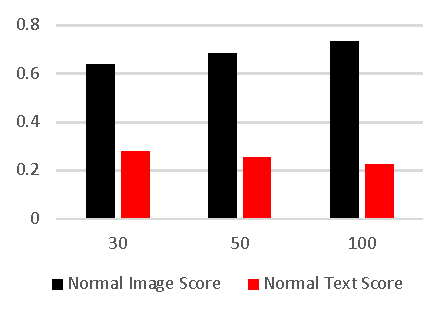
\includegraphics[width=0.45\linewidth]{images/template_length.pdf}
    \label{subfig: different size on}
    }
    \subfigure[Bakcdoor Training]{
    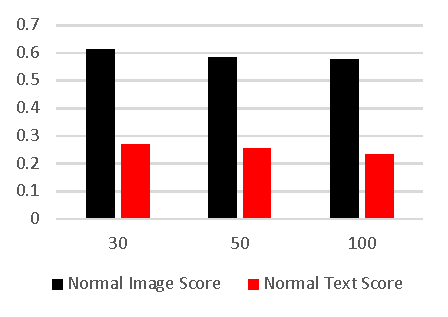
\includegraphics[width=0.45\linewidth]{images/template_length_bc.pdf}
    \label{subfig: different size off}
    }
    \caption{\textbf{Effects of length of the template}. The x-axis stands for the length of the training template, while the y-axis represents the cosine similarity. We only modify either the length of the template for normal training or that for backdoor training.}
    \label{fig:diftarget}
\end{figure}





\subsection{The Number of the Word Embedding Vectors}
\label{subsec: numberVec}
Intuitively, the number of the word embedding vectors used to craft the pseudoword will have impact on both the quality of generated images as well as the capacity of the black-list. This is because the pseudoword has a relatively lower capacity. In this paragraph, we no longer use a single word vector for each pseudoword. Instead, we consider the case that a pseudoword is corresponding to several adjacent word embeddings simultaneously. 

\vspace{.3em}
\noindent \textbf{Influence on normal performance.} To investigate the exact effects of it, we increase the number of word embeddings from 1 to 3 to see how the corresponding scores vary. The results are shown in Fig.~\ref{fig:vector number}. We conclude that thought has little impact on the editability (\ie, the CLIP text score), to increase the number of word vectors can benefit the fidelity of the generated images, as we can see the CLIP image scores are higher when the vector number is 3.

\vspace{.3em}
\noindent \textbf{Influence on the capacity of the blacklist.} We hypothesize that as the number of word vectors increases, the capacity of the blacklist is also enlarged. The expanded feature space is of a higher dimension. Therefore it is more expressive so as to contain more information. From Fig.~\ref{fig:vector number}, we can see that the CLIP image score decreases when we extend the length of the blacklist. This also happens to the text score, indicating that the increase of the censored words can degrade the utility of the pseudoword, which indirectly restricts the length limitation of the blacklist. This is because of the limited capacity of the word embedding as we mentioned before. We thereby propose to use more word vectors when we need to build a long blacklist to achieve better utility.

\section{Conclusion}
We proposed a scalable approach to finetune large language models to follow instructions. Our method leverages large amounts of unlabeled data by developing an iterative self-training algorithm that we dub instruction backtranslation. Our method uses the model itself to both augment  and curate
high quality training examples to improve its own performance. On the Alpaca leaderboard, our finetuned models outperform all other non-distilled instruction-following models, while using fewer human annotated examples.
Future work should scale this method further by considering larger unlabeled corpora, which our analysis suggests should  yield further gains.

% \clearpage


\bibliographystyle{IEEEtran}
\bibliography{references.bib}

% \clearpage
\appendices
\appendix
\section{Sampling from Watershed}
\label{sec: appendix1}

 During training, the sparse optical flow $\mathbf{P}_{d}$ is sampled from the target optical flow. For effective propagation, those guidance vectors should be placed at some keypoints where the motions are representative. We adopt a watershed-based~\citep{zhan2019self} method to sample such keypoints. Given the optical flow of an image, we first extract motion edges using a Sobel filter. Then we assign each pixel a value to be the distance to its nearest edge, resulting in the topological-distance watershed map. Finally, we apply Non-maximum Suppression (NMS) with kernel size $K_f$ on the watershed map to obtain the keypoints. We can adjust $K_f$ to control the average number of sampled points. A larger $K_f$ results in sparser samples. Points on image borders are removed. With the watershed sampling strategy, all the keypoints are roughly distributed on the moving objects.


\begin{figure}[t]
    \centering
    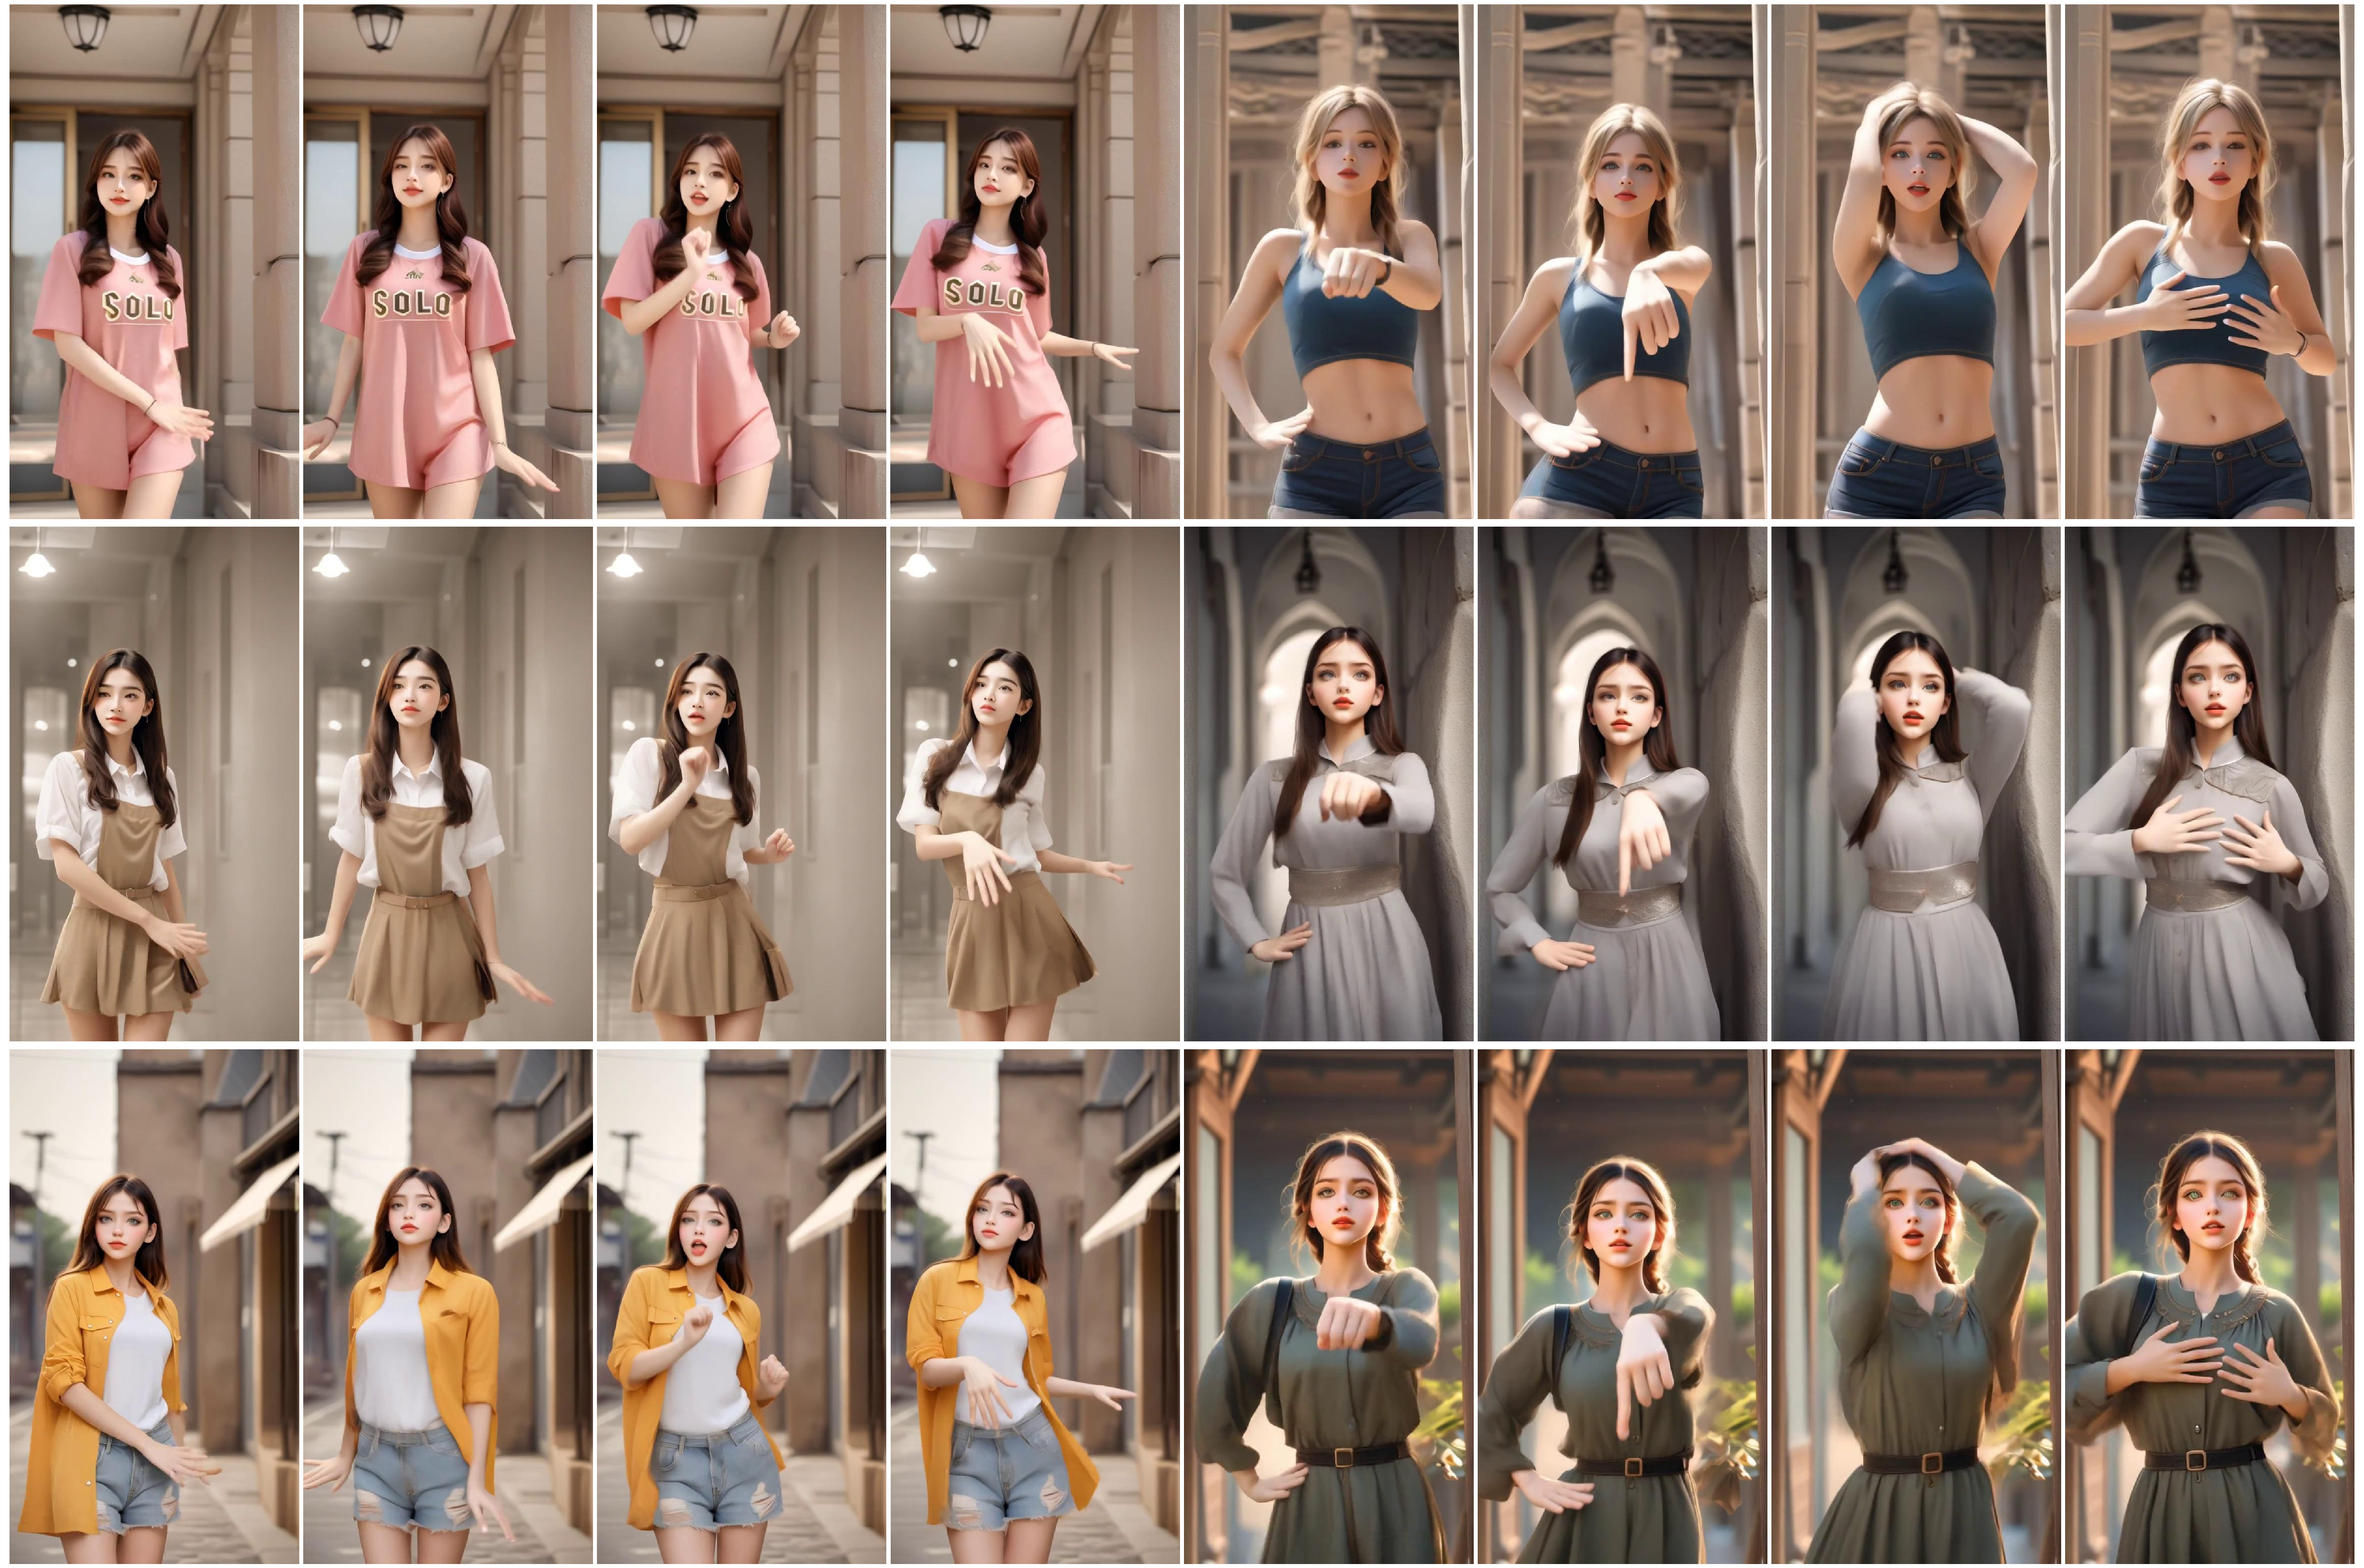
\includegraphics[width=1.0\columnwidth]{./image/appendix_fig1.pdf}
    \vspace{-15pt}
    \caption{More Qualitative Comparisons.}
    \label{fig: appendix_fig1}
\end{figure}

\begin{figure}[t]
    \centering
    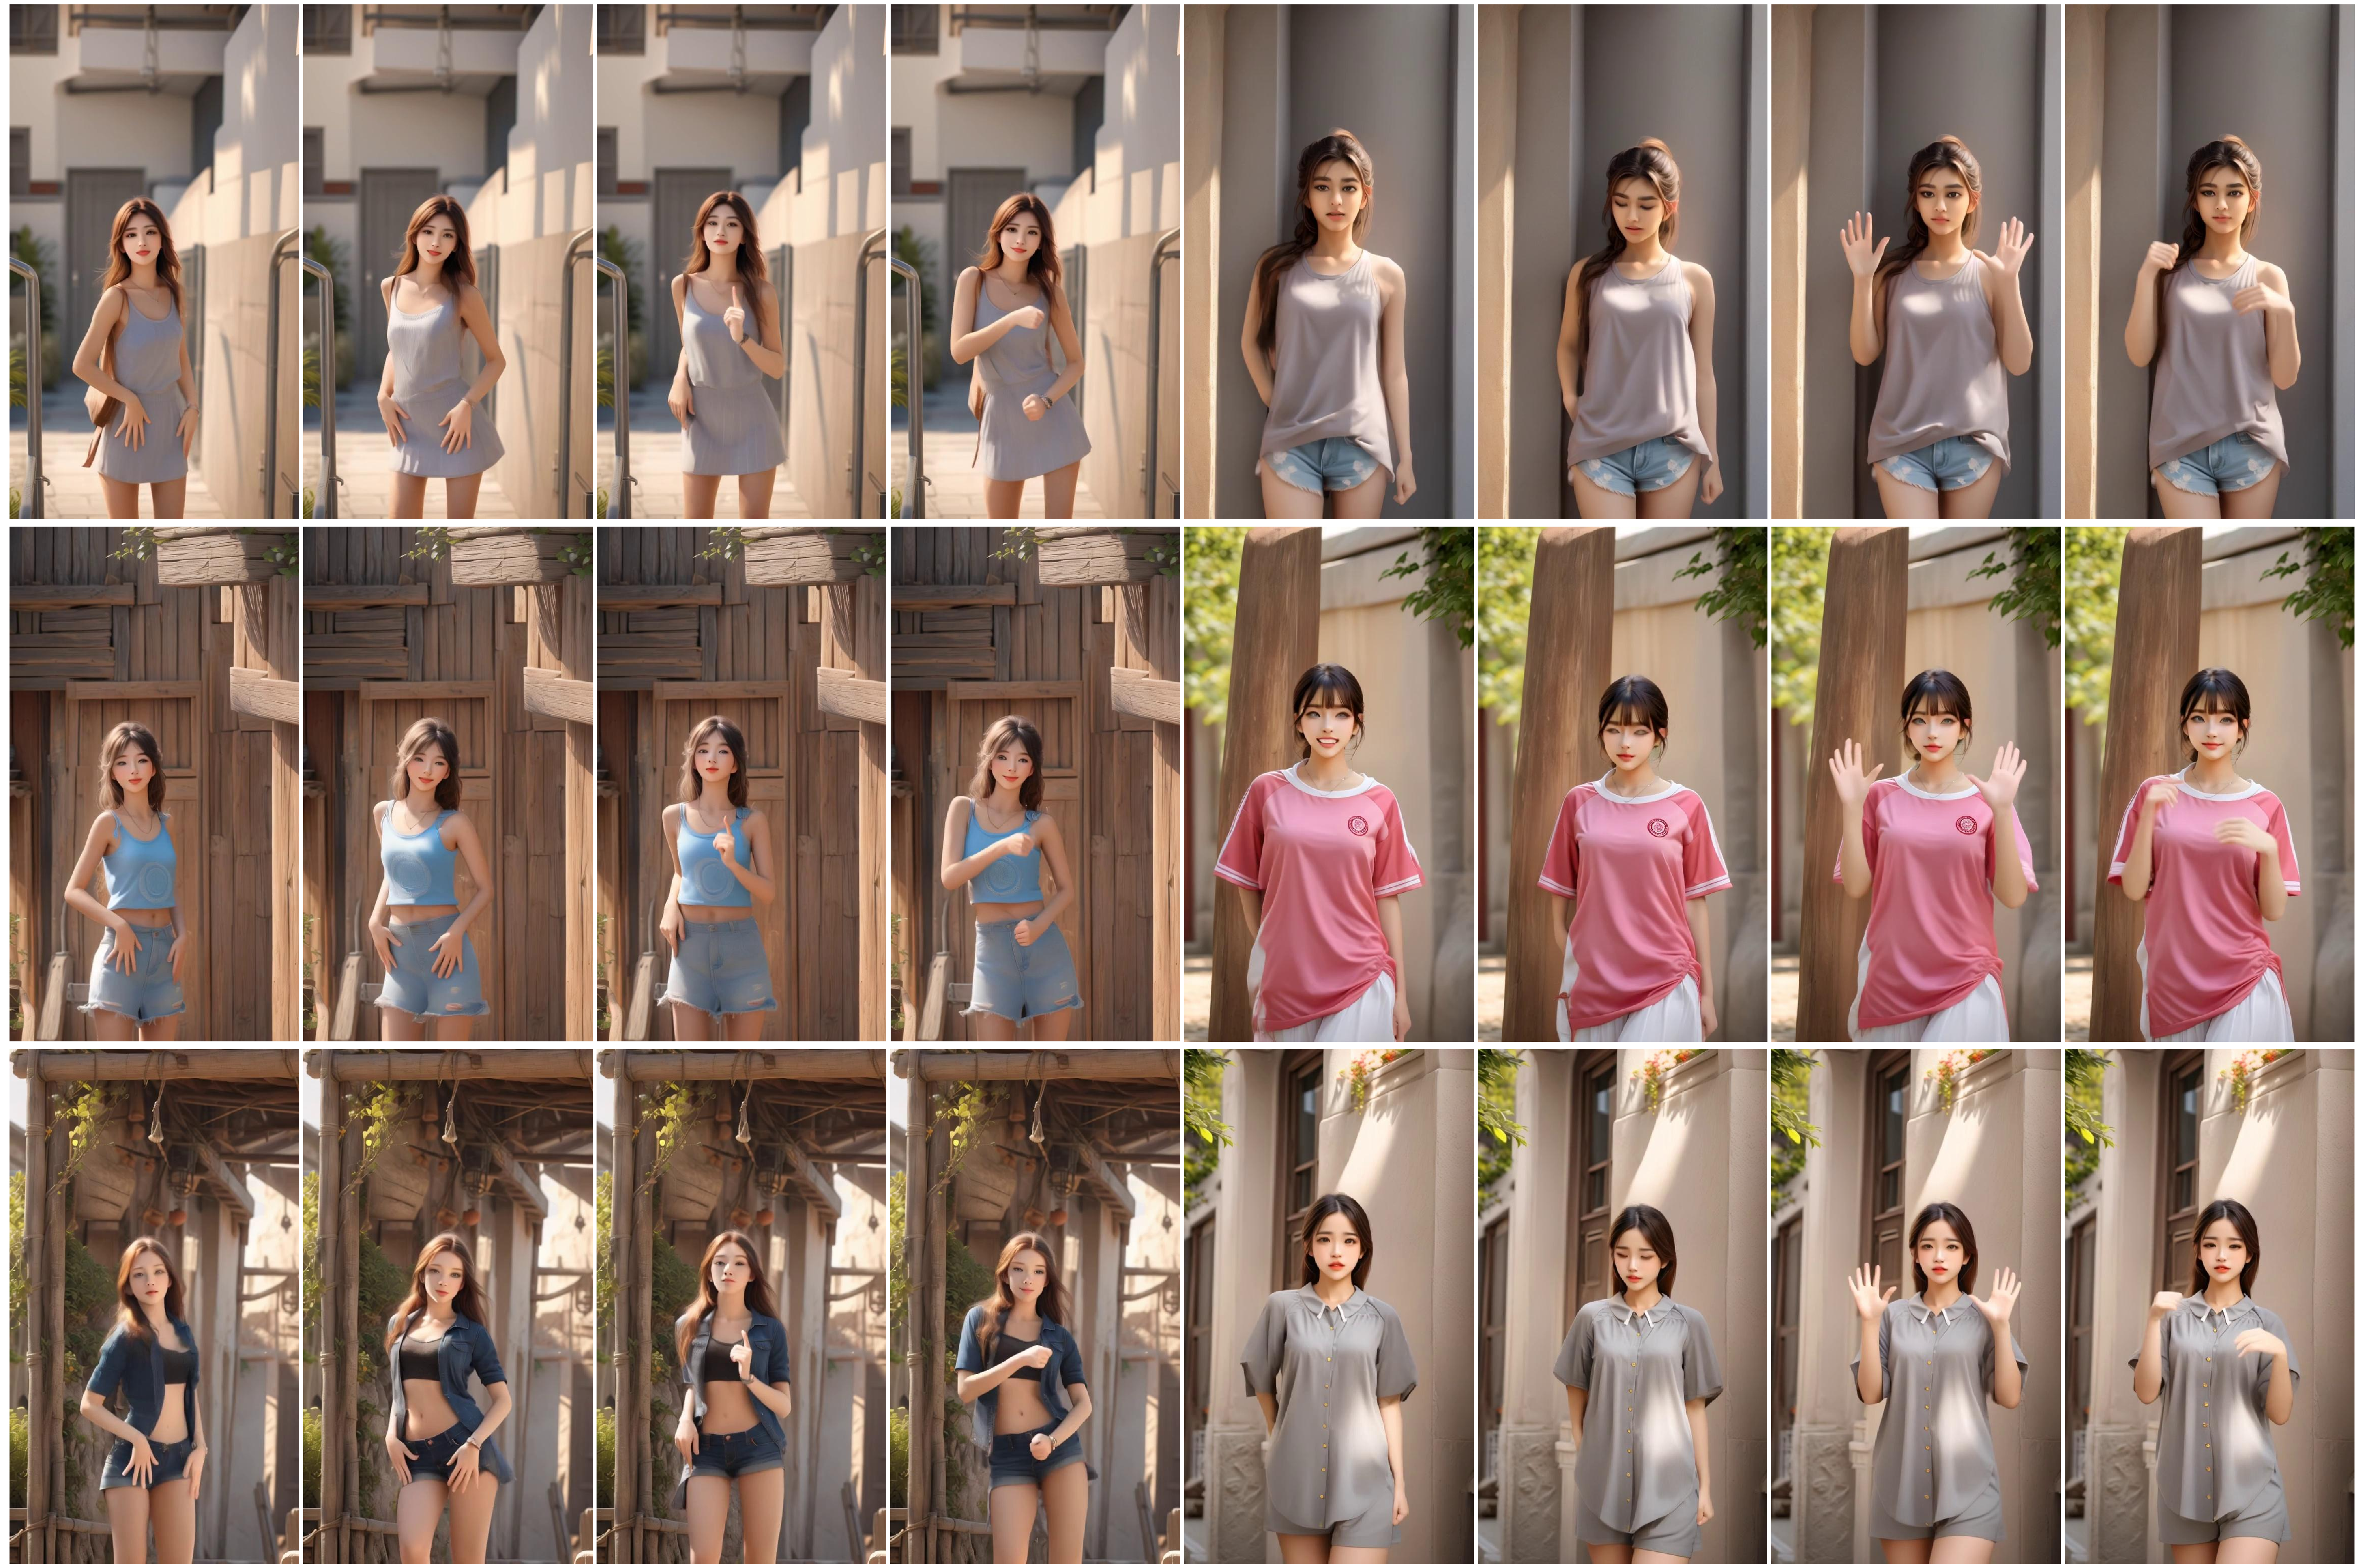
\includegraphics[width=1.0\columnwidth]{./image/appendix_fig2.pdf}
    \vspace{-15pt}
    \caption{More Qualitative Comparisons.}
    \label{fig: appendix_fig2}
\end{figure}
 \section{More Quantitative Results}
 
 Figures~\ref{fig: appendix_fig1} and Figure~\ref{fig: appendix_fig2} illustrate more qualitative results.
\label{sec: more case}

{
\section{More Ablation Analyses}
As shown in Figure~\ref{fig: appendix abs}, the region-level guidance provided by our motion field guidance facilitates the enhancement of consistency across body regions. The proposed keypoints correspondence improves generation quality by aligning DIFT features of the skeleton pose, e.g., facial consistency.
 }

 \begin{figure}[t]
    \centering
    \includegraphics[width=1.0\columnwidth]{./image/abs.png}
    \caption{Qualitative results about motion field guidance and keypoints correspondence.}
    \vspace{-10pt}
    \label{fig: appendix abs}
    
\end{figure}

{
\section{More details of motion field guidance}
There is a gap between the inference and the training optical flow. 
(1) During inference, we do not propose extracting the forward optical flow directly from the driving video, as it ignores the gap between the reference character and the driving video. As shown in Figure~\ref{fig: appendix_flow1}(a)and Figure~\ref{fig: appendix_flow2}(a), directly using the forward optical flow as motion guidance is clearly inconsistent with the reference image.
(2) When there is a large difference between the reference image and the driving video, it is impossible to get the corresponding motion field by the existing optical flow estimation model, as shown in Figure~\ref{fig: appendix_flow2}(b). Therefore, we have to compute Pd differently during inference.
}
{
Although the dense motion field we proposed in Section 4.1 can adapt to different body variations during inference. However, there are two limitations of this dense motion field: (1) there is a gap with the motion field extracted from real videos, and (2) the low computational efficiency is not suitable for use during training. Considering that pairs of training data have no body changes, to utilize accurate control signals during training and to improve computational efficiency, we approximate the optical flow during inference by sampling sparse optical flow before prediction as shown in Figure~\ref{fig: appendix_flow1}(c). 
}

% ############################################
\begin{table*}[t]
\footnotesize
\begin{minipage}[t]{0.33\textwidth}
\centering
\setlength{\tabcolsep}{2pt}
\caption{The impact of hybrid ControlNet.}
% \vspace{-10pt}
\begin{tabular}{lcc}
\toprule
{Methods} & FID-FVD$\downarrow$   & FVD$\downarrow$\\ 
\midrule
Exp1 & 10.43 & 514.83 \\
Exp2 & 10.94 & 551.32 \\
Full Model & 10.24 & 466.93 \\
 \bottomrule
\end{tabular}
\label{tab:appendix_controlnet}
\end{minipage}
\hfill
\begin{minipage}[t]{0.65\textwidth}
\caption{The impact of CMP.}
% \vspace{-10pt}
\centering
\setlength{\tabcolsep}{2pt}
\begin{tabular}{lcc}
\toprule[1pt]
Methods  & subject consistency$\uparrow$ & background consistency$\uparrow$ \\
\midrule
Full Model w/o CMP & 93.94                  &   97.83\\            
Full Model         &94.35                  &  98.75   \\
\bottomrule
\end{tabular}
% \vspace{-1pt}
\label{tab:appendix_cmp}
\end{minipage}
% \vspace{-5pt}
\end{table*}

\begin{table}[t]
% \vspace{-10pt}
\caption{Performance comparisons for image-level metrics.}
\centering
% \setlength{\tabcolsep}{3pt}
\begin{tabular}{lcccc}
\toprule
Methods  & SSIM $\downarrow$ & PSNR$\downarrow$ & LPIPS$\uparrow$  & L1$\uparrow$ \\
\midrule
MusePose &0.788& 19.14&  0.263&  2.46E-05\\     
MusePose+Ours  &0.811  &19.36  &0.238  &2.26E-05\\
\midrule
MimicMotion &0.749  &18.32  &0.272& 2.71E-05\\
MimicMotion+Ours & 0.781&19.58 &0.242&2.42E-05 \\
\bottomrule
\label{tab:appendix_exp}
\end{tabular}
\end{table}

\begin{table}[t]
% \vspace{-10pt}
\caption{Performance comparisons for image-level metrics.}
\centering
% \setlength{\tabcolsep}{3pt}
\begin{tabular}{lcc}
\toprule
Methods  & trainable parameters(MB) & infer time (sec/frame) \\
\midrule
MusePose	&2072.64	&3.37 \\
MimicMotion	&1454.19	&1.61 \\
MimicMotion+Ours	&653.4	&2.36\\
\bottomrule
\label{tab:appendix_eff}
\end{tabular}
\end{table}

{
\section{More Ablation Study}
\subsection{The impact of hybrid ControlNet architecture}
We show the impact of hybrid ControlNet architecture in Table~\ref{tab:appendix_controlnet}. Specifically, we design two variant architectures, (1) Exp1: inserting the motion field into the denoising network instead of the hybrid controller as shown in Figure~\ref{fig: appendix_abs_pipeline}(a), and (2) Exp2: removing the hybrid ControlNet and inserting the motion field guidance and keypoint correspondence into the denoising network as shown in Figure~\ref{fig: appendix_abs_pipeline}(b). Exp1 shows that the motion field needs to be jointly optimized with U-Net to provide the correct representation. Exp2 shows that complex motion information and appearance features cannot be modeled with only two shallow encoders.
}
{
\subsection{The impact of CMP.}
We provide the ablation analysis of CMP in Table~\ref{tab:appendix_cmp}, which shows that CMP can improve the consistency of the generated video.
}

\begin{figure}[h!]
    \centering
    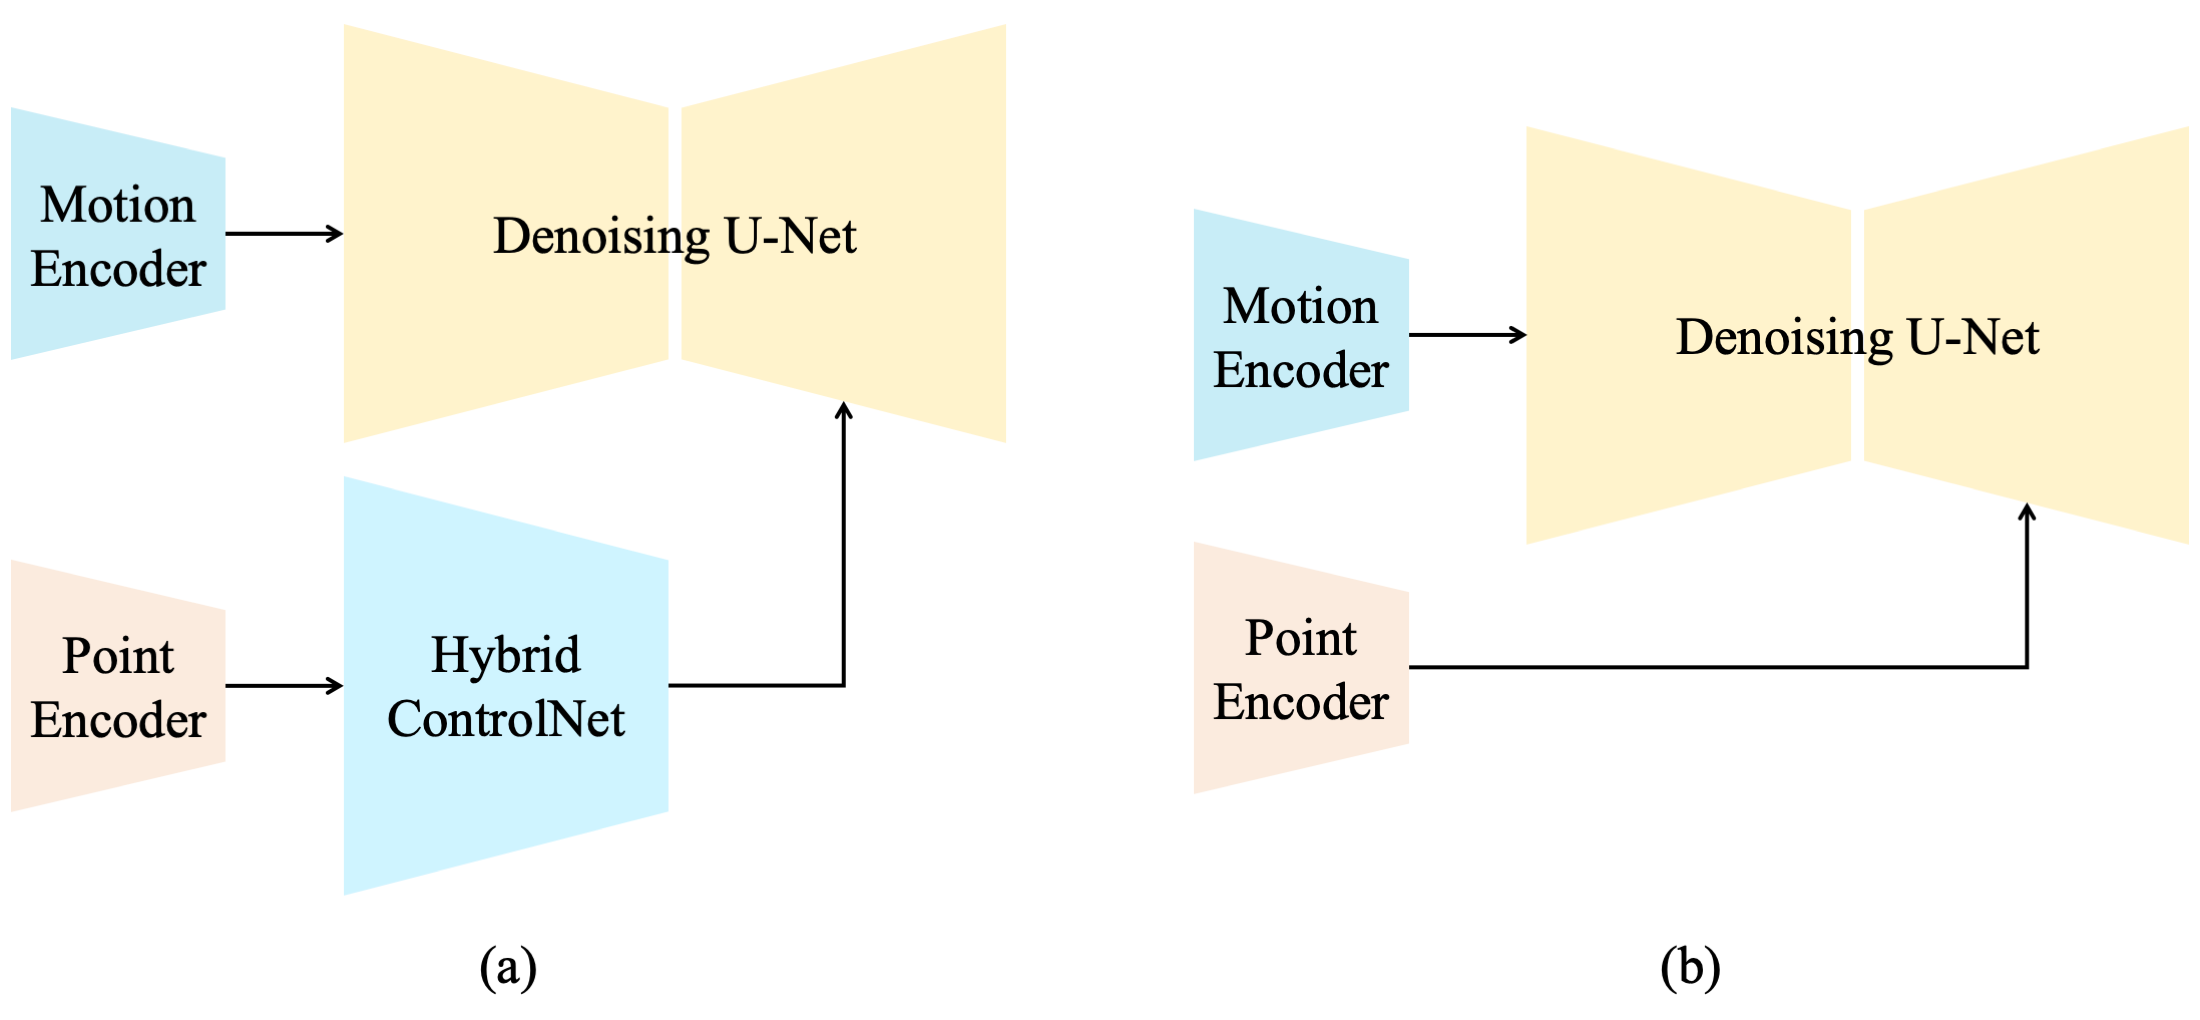
\includegraphics[width=.9\columnwidth]{./image/abs_pipeline.png}
    \vspace{-15pt}
    \caption{Different hybrid ControlNet architectures.}
    \label{fig: appendix_abs_pipeline}
\end{figure}

{
\section{More Performance Comparisons.}
To further evaluate the generated results, we provide performance comparisons for image-level metrics in Table~\ref{tab:appendix_exp}. Compared to the baseline model, our method achieves significant improvements in all metrics.
}
{
\section{Trainable Parameters and Inference Time}
We compare the trainable parameters and inference time of the different models in Table~\ref{tab:appendix_eff}. For a fair comparison, the size of the generated video is set to 576x1024. Our method requires fewer trainable parameters based on the baseline model.
During inference, our method estimates the motion field for the reference image, which increases inference time a little.
}

{
\section{Analysis of Background Noise.}
Since our motion fields are not extracted directly from the driving video, some noise due to estimation errors may be introduced. As shown in Figure~\ref{fig: appendix_flow_noise}, the motion field of the reference image without the background is more accurate than the complex background.
}

\begin{figure}[t]
    \centering
    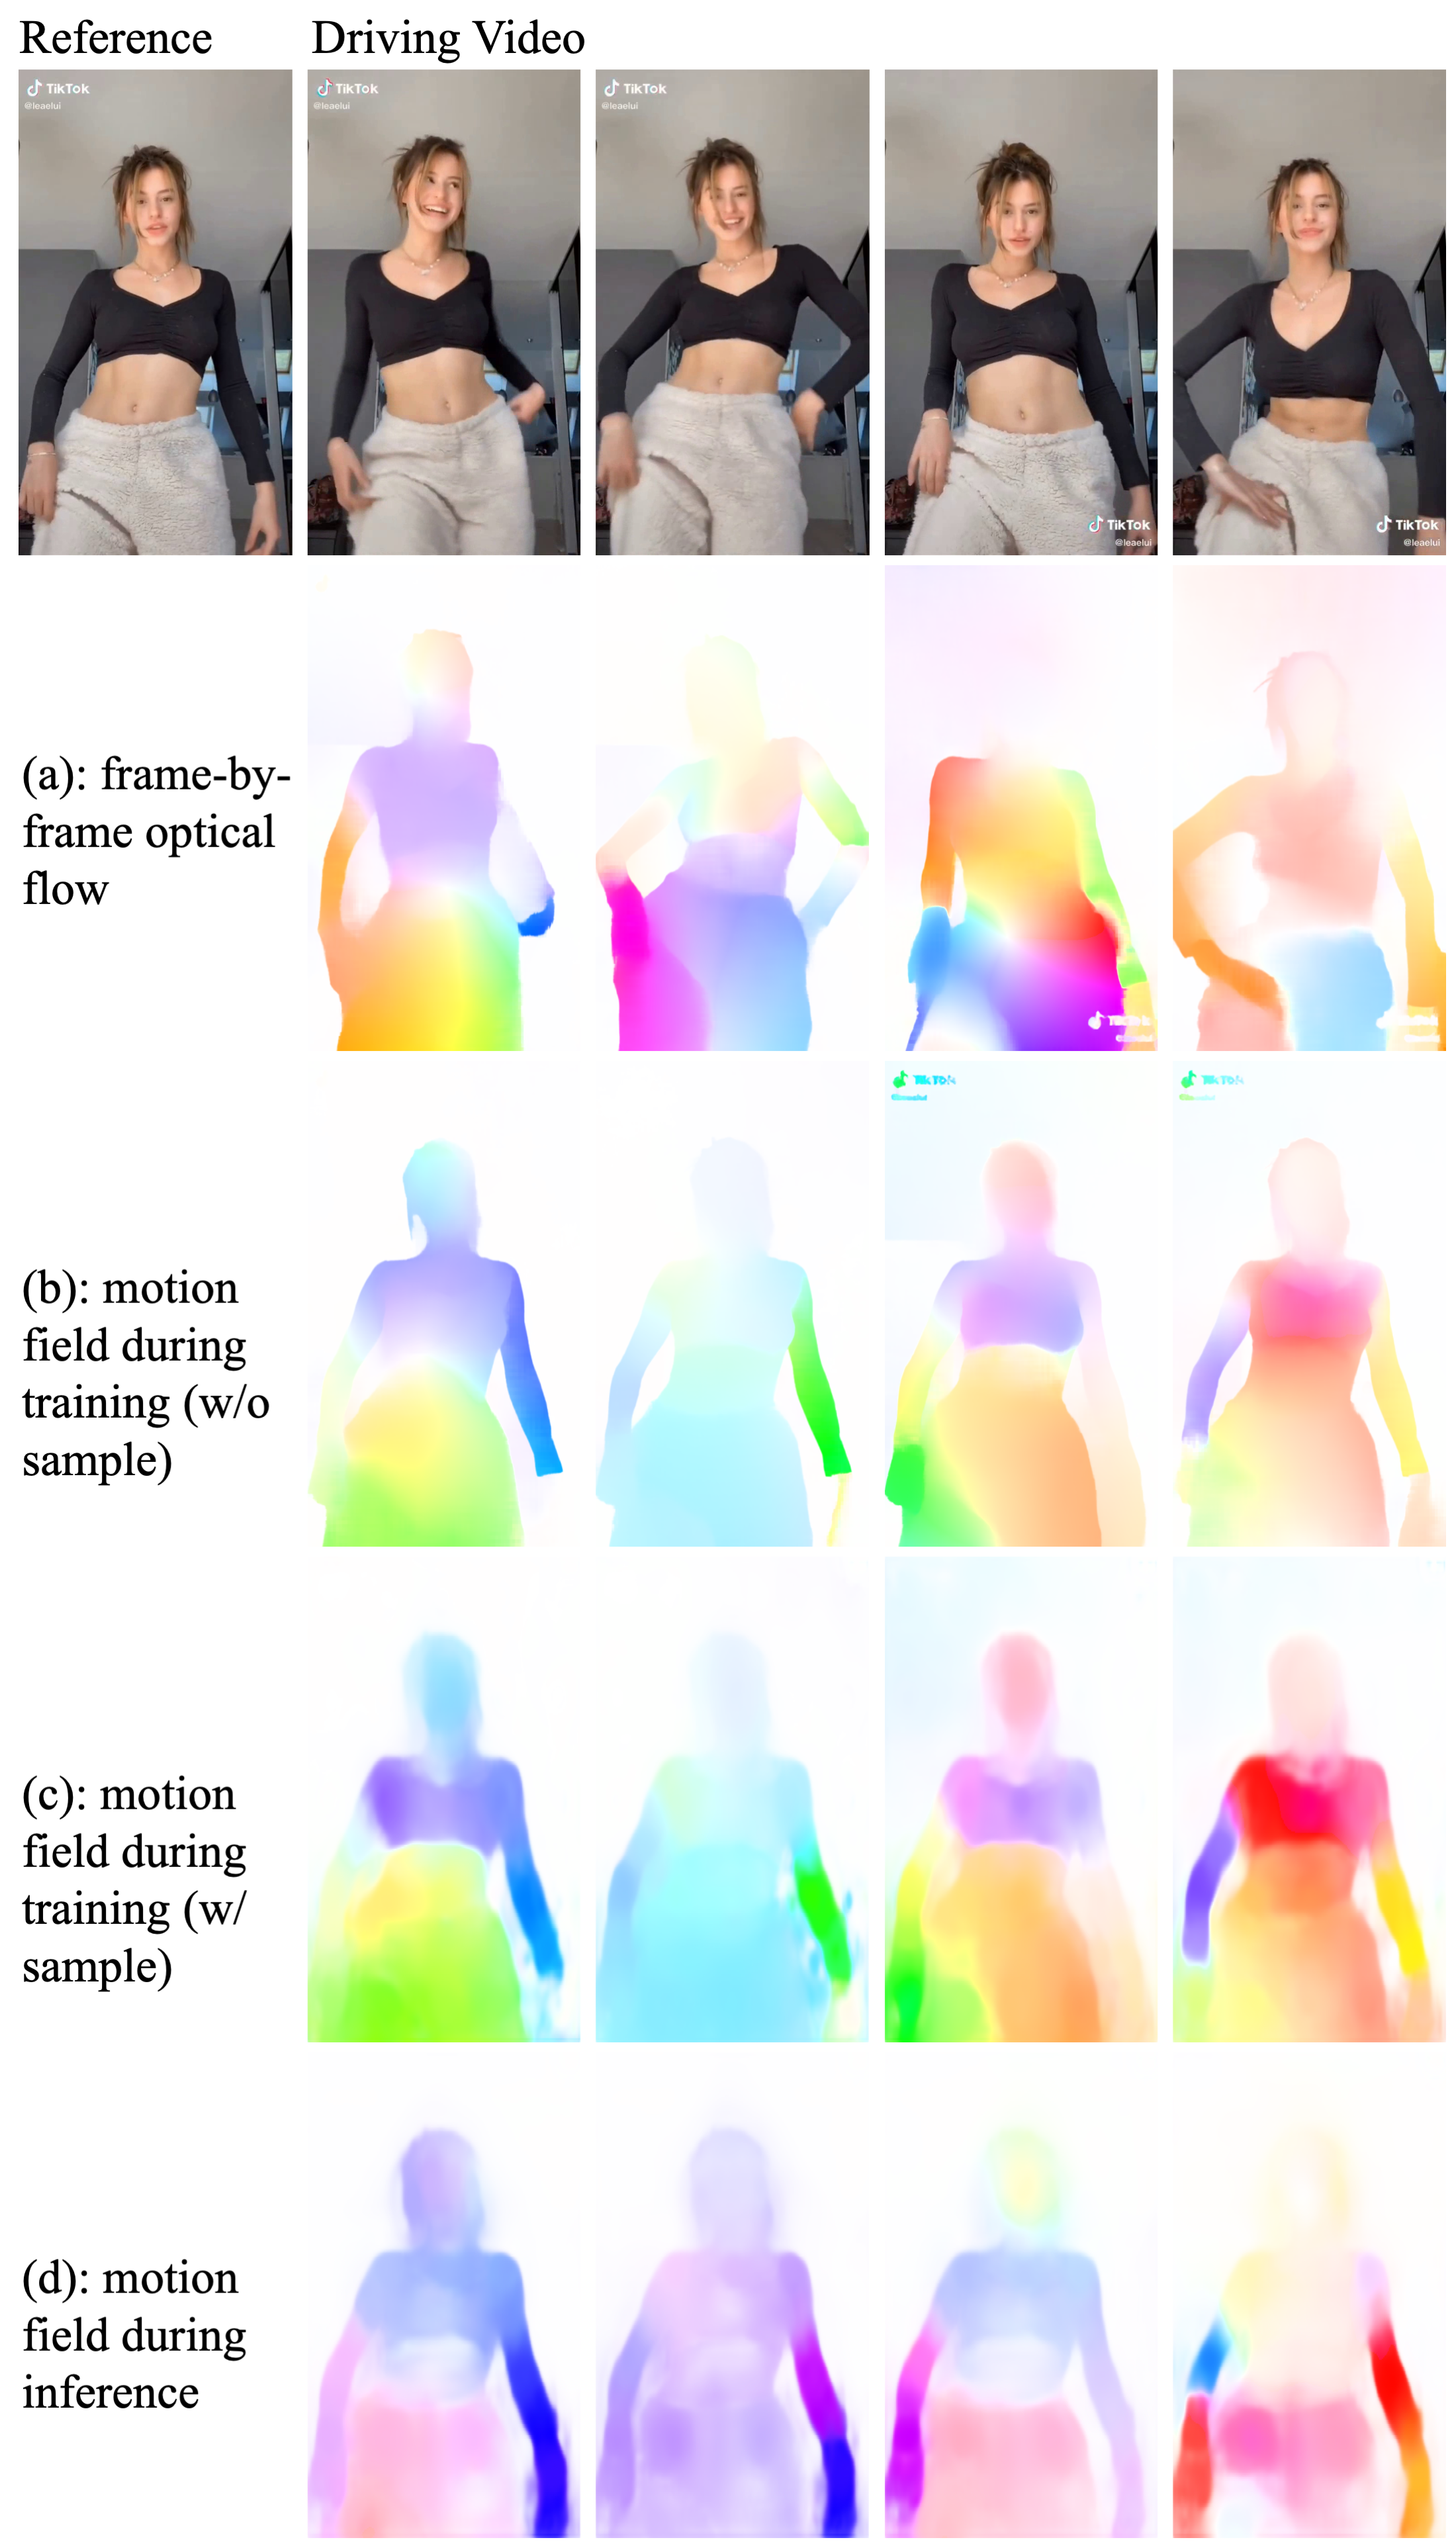
\includegraphics[width=.9\columnwidth]{./image/flow1.png}
    \vspace{-10pt}
    \caption{Body matched motion field visualization.}
    \label{fig: appendix_flow1}
\end{figure}

\begin{figure}[t]
    \centering
    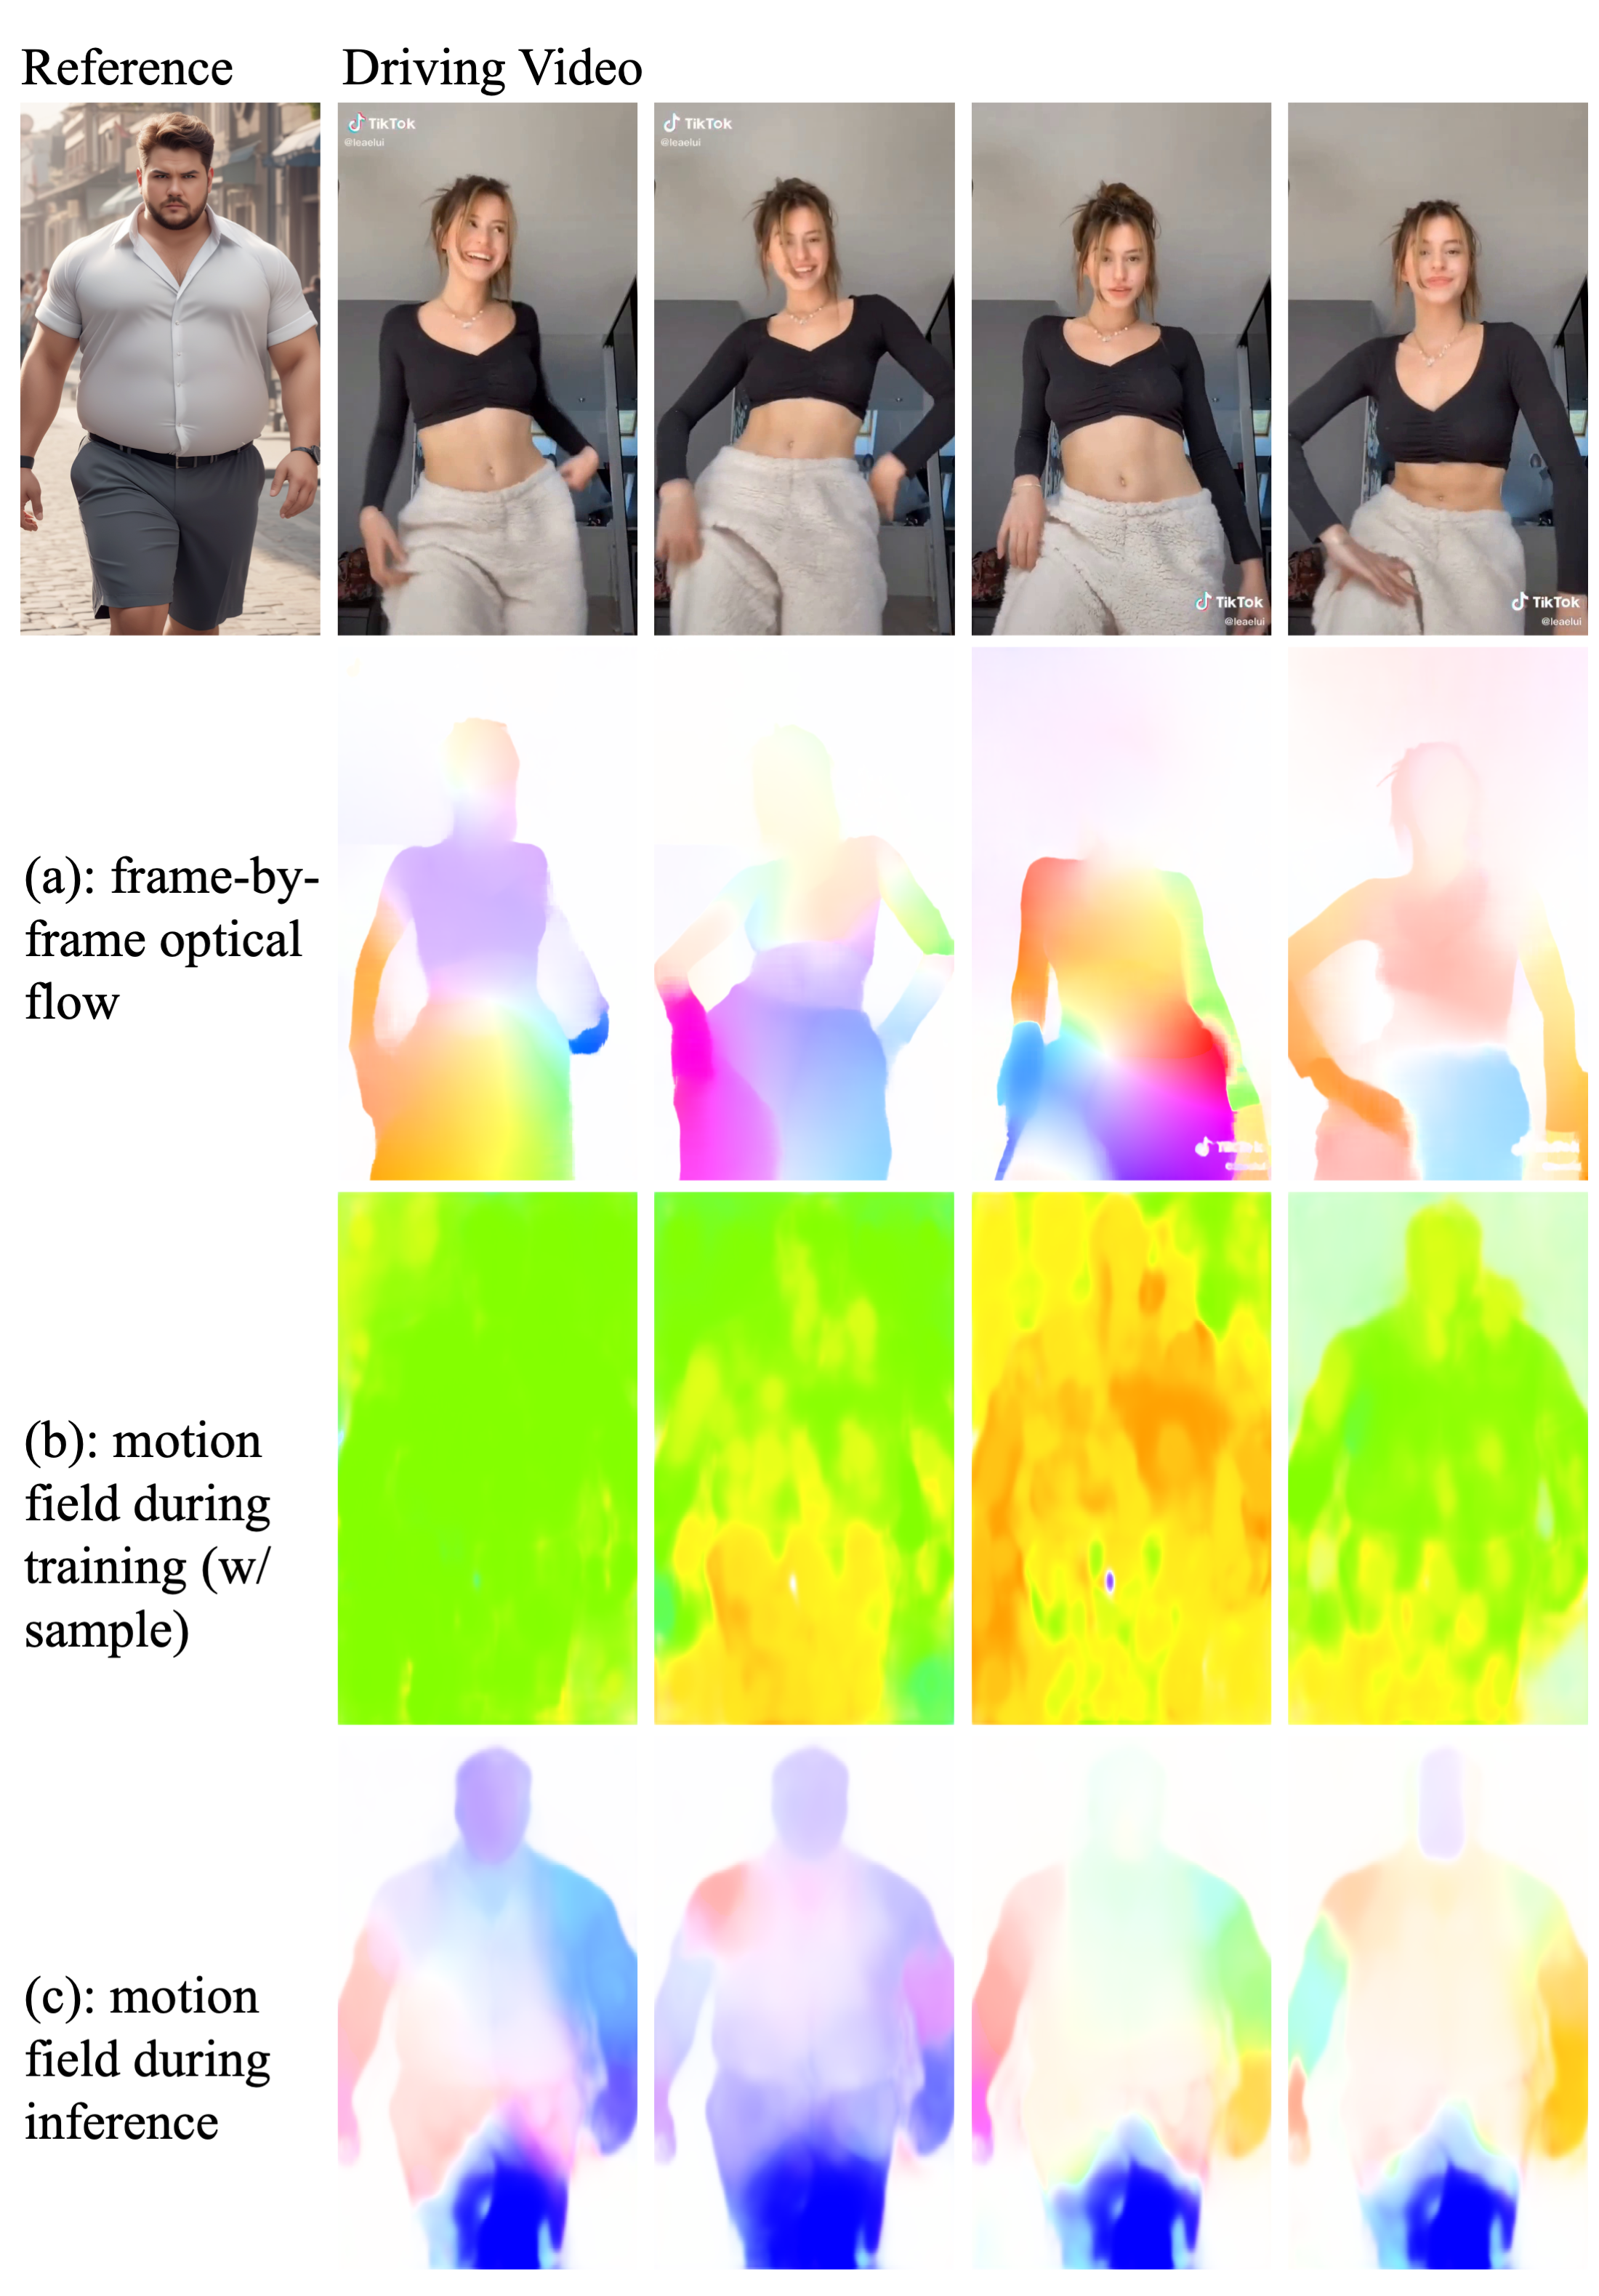
\includegraphics[width=.9\columnwidth]{./image/flow2.png}
    \vspace{-10pt}
    \caption{Body mismatched motion field visualization.}
    \label{fig: appendix_flow2}
\end{figure}

\begin{figure}[t]
    \centering
    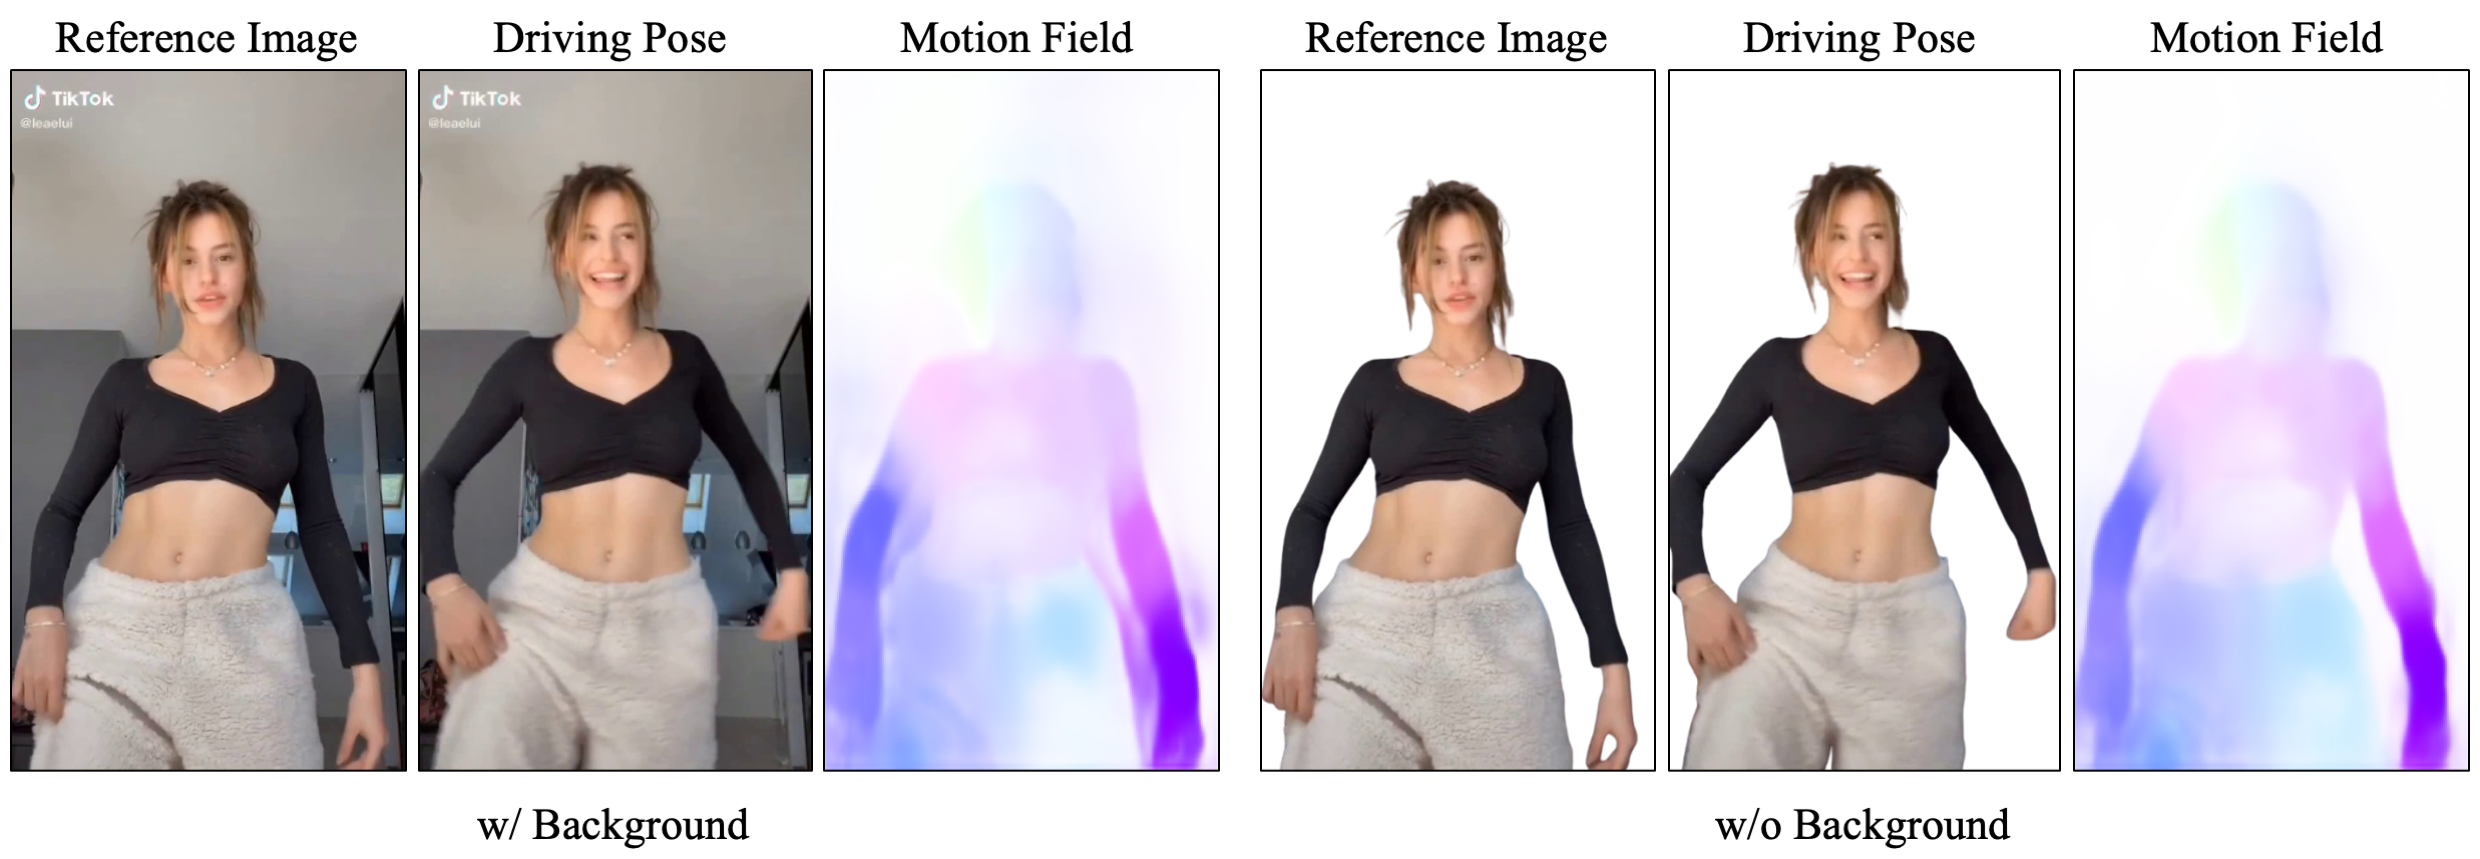
\includegraphics[width=.9\columnwidth]{./image/flow_noise.png}
    \vspace{-10pt}
    \caption{Analysis of background noise.}
    \label{fig: appendix_flow_noise}
\end{figure}

\end{document}
